\documentclass[10pt,fleqn,a4paper]{jsarticle}
\usepackage[dvipdfmx]{graphicx,color}
\usepackage{ascmac,amsmath,amssymb,amstext}
\usepackage{tikz,multicol,float,tikz-3dplot}
\usetikzlibrary{positioning,intersections,calc,arrows.meta,math,angles}
\usepackage{zogeny,ceo,comment}
\newcommand{\ans}[1]{\mbox{\boldmath{$#1$}}}
\renewcommand{\baselinestretch}{1.3} 
\tdplotsetmaincoords{60}{110}%{xy平面からどれだけ上にいるか(90度から-90度)}{z軸中心にどれだけ左右に回転するか}
\title{早稲田大学ー社会科学部ー過去問演習と良問演習}
\author{大島 遙斗}
\begin{document}
\maketitle
\newpage
{\LARGE はじめに}\\
長い長い受験勉強もとうとう終わりが見えてきました.今これを書いているのは12月の14日の深夜です.今から,2ヶ月後の理瀬さんは
もう大学入試を終えています.さて,どんな景色が見えているのでしょうか.\\\\
今から志望校の合格にできることは,たくさん問題をといてパターンをたくさん身につけるのではなく,
\begin{center}
\ans{出会った問題から何を学ぶか?}
\end{center}です.\\
1日1日を大切に頑張っていきましょう.\\\\
また,勉強の相談やメンタル的にしんどいなどあれば気軽に電話なり,直接僕に話しかけたりして教えてください!いつでも相談にのります!最終局面に向けて
一緒に頑張りましょう.\\
\hspace{14cm}大島 遙斗
\newpage
\begin{center}
    {\LARGE 本書の使い方}
\end{center}
まず,このテキストは\ans{早稲田の三年分の過去問と僕が選んだ良問}の二部から構成されています.\\
それぞれ1週間のうちに解いてきてください.\\
・過去問について\\
 言わずもがなよく復習してください.何がダメで次はどうすれば解けるようになるのか,どのような発想があったら解くことができていたのか,
を考えながら復習しましょう.\\
・良問について\\
 立教が一応のところの第一志望だと思うので掲載する問題は,\hyoujyun 〜\yayanan の問題を集めます.また,以下の記号を用います.\\
A$\to 基本的な問題.教科書レベル.\\
B\to 標準的な問題.ぜひ解き切って欲しい問題.\\
C\to $難問.この問題が解けなくても,周りの受験生とはあまり差がつかない.\\
 例えば,次のように問題の横に書いたら次のように捉えてください.\\
\kagil B15\kagir$=$標準的な問題で目標解答時間は,15分\\
また,本題の他に\fbox{\kurosankakub 類題演習\kurosankakua}というものを掲載します.必ずしも解いてくる必要はありません.自分の実力向上に役立ててください.
\newpage
\tableofcontents
\newpage
\section{早稲田大学過去問題編}
\subsection{2023年実施}
\begin{center}
    {\LARGE 2023年度:数学}
\end{center}
\begin{center}
{\LARGE 注意事項}\\
\end{center}
1. 試験開始の合図があるまで,問題冊子及び記述解答用紙には手を触れないこと.\\
2. 問題は\ans{10〜11ページ}に記載されている.試験中に問題冊子の印刷不鮮明,ページの落丁・乱丁及び解答用紙の汚損等に気づいた場合
は,手を挙げて試験員に知らせること.\\
3. 解答はすべて,HBの黒鉛筆またはHBのシャープペンシルで記入すること.\\
4. 記述解答用紙記入上の注意\\
  \kakkoichi  試験開始後,記述解答用紙の所定欄(2箇所)に,氏名及び受験番号を正確に記入すること.\\
  \kakkoni 所定欄以外に受験番号・氏名を記入した解答用紙は採点の対象外となる場合はある.\\
  \kakkosan 受験番号の記入にあたっては,次の数字見本にしたがい,読みやすいように,正確に記入すること.\\
  \kakkoshi 受験番号は右詰めで記入し,余白が生じる場合でも受験番号の前に「0」を記入すること.\\
  \kakkogo 計算の途中過程を記述すること.記述されていない答案は採点の対象外になる場合がある.\\
  \kakkoroku 定規,コンパスを使用してもよい.\\
5. あとは\\
6. なんだかんだ\\
7. 色々と\\
8. 注意事項が\\
9. 書いてあります.\\
\newpage
\begin{center}
    計算用紙
\end{center}
\newpage
\begin{center}
    計算用紙
\end{center}
\newpage
\begin{center}
    計算用紙
\end{center}
\newpage
\begin{center}
    計算用紙
\end{center}
\newpage
\noindent
\reibanichi\\
 曲線$y=ax^2+b上にx座標がpである点Pをとり,点Pにおける接線を\ell とする.$\\
ただし,定数$a,bはa>0,b>0を満たすとする.次の問に答えよ.$\\\\
\kakkoichi 接線$\ell の方程式をa,b,pを用いて表せ.\\
\kakkoni  接線\ell とy=ax^2で囲まれた部分の面積Sをa,bを用いて表せ.\\
\kakkosan 接線\ell と曲線y=ax^2+\dfrac{b}{2}で囲まれた図形の面積をS^\prime としたとき,S^\prime をSを用いて表せ.\\
\kakkoshi 接線\ell と曲線y=ax^2+cで囲まれた部分の面積S^{\prime\prime} とする.S^{\prime\prime}=\dfrac{S}{2}のとき,
cをa,bを用いて表せ.ただし,b>cとする.$\\\\\\\\\\\\\\\\\\\\
\reibanni\\
 定数$mに対してx,y,zの方程式$
\begin{center}
    $xyz+x+y+z=xy+yz+zx+m\hspace{2cm}\cdots\maruichi$
\end{center}
を考える.次の問に答えよ.\\\\
\kakkoichi $m=1のとき\maruichi 式をみたす実数x,y,zの組をすべて求めよ.$\\
\kakkoni $m=5のとき\maruichi 式を満たす実数x,y,zの組をすべて求めよ.ただし,x\leq y\leq zとする.$\\
\kakkosan $xyz=x+y+zを満たす整数x,y,zの組をすべて求めよ.ただし,0<x\leq y\leq zとする.$
\newpage
\reibansan\\
 $a=\sqrt[3]{5\sqrt{2}+7}-\sqrt[3]{5\sqrt{2}-7}とする.次の問に答えよ.$\\\\
\kakkoichi $a^3をaの1次式で表せ.$\\
\kakkoni $aは整数であることを示せ.$\\
\kakkosan $b=\sqrt[3]{5\sqrt{2}+7}+\sqrt[3]{5\sqrt{2}-7}とするとき,bを超えない最大の整数を求めよ.$\\\\\\\\
\begin{center}
    {\LARGE\kagil 以 下 余 白\kagir}
\end{center}
\newpage
\subsection{2024年度実施}
\begin{center}
    {\LARGE 2024年度:数学}
\end{center}
\begin{center}
{\LARGE 注意事項}\\
\end{center}
1. 試験開始の合図があるまで,問題冊子及び記述解答用紙には手を触れないこと.\\
2. 問題は\ans{17〜18ページ}に記載されている.試験中に問題冊子の印刷不鮮明,ページの落丁・乱丁及び解答用紙の汚損等に気づいた場合
は,手を挙げて試験員に知らせること.\\
3. 解答はすべて,HBの黒鉛筆またはHBのシャープペンシルで記入すること.\\
4. 記述解答用紙記入上の注意\\
  \kakkoichi  試験開始後,記述解答用紙の所定欄(2箇所)に,氏名及び受験番号を正確に記入すること.\\
  \kakkoni 所定欄以外に受験番号・氏名を記入した解答用紙は採点の対象外となる場合はある.\\
  \kakkosan 受験番号の記入にあたっては,次の数字見本にしたがい,読みやすいように,正確に記入すること.\\
  \kakkoshi 受験番号は右詰めで記入し,余白が生じる場合でも受験番号の前に「0」を記入すること.\\
  \kakkogo 計算の途中過程を記述すること.記述されていない答案は採点の対象外になる場合がある.\\
  \kakkoroku 定規,コンパスを使用してもよい.\\
5. あとは\\
6. なんだかんだ\\
7. 色々と\\
8. 注意事項が\\
9. 書いてあります.\\
\newpage
\begin{center}
    計算用紙
\end{center}
\newpage
\begin{center}
    計算用紙
\end{center}
\newpage
\begin{center}
    計算用紙
\end{center}
\newpage
\begin{center}
    計算用紙
\end{center}
\newpage
\noindent\reibanichi \\
連立不等式\\
\begin{center}
    $y\leq-\dfrac{2}{3}x+4,   y\geq x-1,   x\geq0,   y\geq0$
\end{center}
の表す領域を$Dとする.点(x,y)がDを動くとき,次の問に答えよ.$\\\\
\kakkoichi $領域Dを座標平面上に図示せよ.$\\
\kakkoni $-2x+yの最大値と,そのときのx,yの値を求めよ.$\\
\kakkosan $2x+yの最大値と,そのときのx,yの値を求めよ.$\\
\kakkoshi $aがすべての実数を動くとき,ax+yの最大値をaで分類せよ.$\\\\\\\\\\\\\\\\\\
\reibanni\\
 $\mathrm{OA}=6,\mathrm{OB}=5,\mathrm{AB}=7である\Sankaku{OAB}について,\vec{a}=\Vec{OA},\vec{b}=\Vec{OB}とおく.
次の問に答えよ.$\\\\
\kakkoichi $\Sankaku{OAB}の内心を\mathrm{I},辺\mathrm{AB}と直線\mathrm{OI}の交点をCとする.\Vec{OC}を\vec{a},\vec{b}で表せ.$\\
\kakkoni $\Vec{OI}を\vec{a},\vec{b}で表せ.$\\
\kakkosan 内積$\vec{a}\cdot\vec{b}の値を求めよ.$\\
\kakkoshi $\Sankaku{OAB}の垂心を\mathrm{H},\Vec{OH}=s\vec{a}+t\vec{b}とするとき,\Vec{AH},\Vec{BH}を\vec{a},\vec{b},s,tで表せ.$\\
\kakkogo $s,tの値を求めよ.$
\newpage
\noindent\reibansan\\
 $nをn\geq3 である自然数とする.相異なるn個の正の数を小さい順に並べた集合S=\B{a_1,a_2,\cdots,a_n}を考える.a_1=kとする
とき,次の問に答えよ.$\\\\
\kakkoichi $a_i-a_1(i=2,3,\cdots,n)がすべてSの要素となるとき,a_2を求めよ.$\\
\kakkoni \kakkoichi のとき,$a_nをnで表せ.$\\
\kakkosan $\dfrac{a_i}{a_1}(i=2,3,\cdots,n)がすべてSの要素となるとき,a_nをnの式で表せ.$\\\\\\\\
\begin{center}
    {\LARGE\kagil 以 下 余 白\kagir}
\end{center}
\newpage
\subsection{2025年度実施}
\begin{center}
    {\LARGE 2025年度:数学}
\end{center}
\begin{center}
{\LARGE 注意事項}\\
\end{center}
1. 試験開始の合図があるまで,問題冊子及び記述解答用紙には手を触れないこと.\\
2. 問題は\ans{24〜25ページ}に記載されている.試験中に問題冊子の印刷不鮮明,ページの落丁・乱丁及び解答用紙の汚損等に気づいた場合
は,手を挙げて試験員に知らせること.\\
3. 解答はすべて,HBの黒鉛筆またはHBのシャープペンシルで記入すること.\\
4. 記述解答用紙記入上の注意\\
  \kakkoichi  試験開始後,記述解答用紙の所定欄(2箇所)に,氏名及び受験番号を正確に記入すること.\\
  \kakkoni 所定欄以外に受験番号・氏名を記入した解答用紙は採点の対象外となる場合はある.\\
  \kakkosan 受験番号の記入にあたっては,次の数字見本にしたがい,読みやすいように,正確に記入すること.\\
  \kakkoshi 受験番号は右詰めで記入し,余白が生じる場合でも受験番号の前に「0」を記入すること.\\
  \kakkogo 計算の途中過程を記述すること.記述されていない答案は採点の対象外になる場合がある.\\
  \kakkoroku 定規,コンパスを使用してもよい.\\
5. あとは\\
6. なんだかんだ\\
7. 色々と\\
8. 注意事項が\\
9. 書いてあります.\\
\newpage
\begin{center}
    計算用紙
\end{center}
\newpage
\begin{center}
    計算用紙
\end{center}
\newpage
\begin{center}
    計算用紙
\end{center}
\newpage
\begin{center}
    計算用紙
\end{center}
\newpage
\noindent\reibanichi\\
 $自然数n,pに対して,n^pの1の位の数をf_p(n)で表す.次の問に答えよ.$\\\\
\kakkoichi $f_2(n)の取りうる値をすべて求めよ.$\\
\kakkoni $f_5(n)-f_1(n)の値をすべて求めよ.$\\
\kakkosan $f_{100}(n)の取りうる値をすべて求めよ.$\\\\\\\\\\\\\\\\\\\\\\\\
\reibanni\\
 数列$\B{a_n}の階差数列を\B{B_n},すなわち,$
\begin{center}
    $b_n=a_{n+1}-a_n   (n=1,2,3,\cdots)$
\end{center}
とする.次の問に答えよ.\\\\
\kakkoichi $a_n=-\dfrac{1}{n}のとき,b_mをnの式で表せ.$\\
\kakkoni $b_n=\dfrac{1}{n(n+1)}のとき,a_nをnの式で表せ.$\\
\kakkosan $数列\B{b_n}が以下を満たすときa_nをnの式で表せ.ただし,a_1=1とする.$
\begin{center}
    $\begin{cases}
        b_1=1\\
        b_n=n(n+1) (n\geq2)
    \end{cases}$
\end{center}
\newpage
\noindent\reibansan\\
 $\theta の関数$
\begin{center}
$f(\theta)=\cos2\theta-\sqrt{3}\sin2\theta+4\cos\frac{\theta}{2}\p{\sin\frac{\theta}{2}-\sqrt{3}\cos\frac{\theta}{2}+2\sqrt{3}}$
\end{center}
を考える.ただし,$0\leq\theta\pi とする.次の問に答えよ.$\\\\
\kakkoichi $k=\sin\theta-\sqrt{3}\cos\theta とおくとき,f(\theta)をkの関数で表せ.$\\
\kakkoni $f(\theta)の最大値,最小値をも求めよ.また,そのときの\theta の値を求めよ.$\\
\kakkosan $\kakkoichi のkに対して,\theta の方程式f(\theta)=akの解の個数を求めよ.ただし,定数aは0<a\leq3とする.$\\\\\\\\
\begin{center}
    {\LARGE\kagil 以 下 余 白\kagir}
\end{center}
\newpage



\section{良問集問題編}
\subsection{第1回}
まずは,単純な計算問題で肩慣らしといきましょう.おっとその前に公式の確認です.\\
\koushikia\\
\doichi  $\ans{|X|=k\doti X=\pm kかつk\geq0}\\
\doni \ans{|X|<k\doti -k<X<k}\\
\dosan \ans{|X|>k\doti X>kまたはX<-k}$\\
\begin{itembox}
[l]{\noindent\ba{1.0}.\kagil 絶対値と不等式(A10)\kagir}
以下の不等式をそれぞれ解け.\\
\kakkoichi $|x+3|\geq|x-2|$\hspace{7cm}(25 宮崎大・教,農)\\%bunkei-49
\kakkoni $|4x-1|<|x+3|$\hspace{7cm}(25 福島大)%bunkei-50
\end{itembox}\\\\\\\\\\\\\\\\\\\\\\

\begin{itembox}
    [l]{\fbox{\kurosankakub 類題演習1.1\kurosankakua}}
\kakkoichi 不等式$|2x-3|\leq2の解を求めよ.さらに,不等式|2x-3|\leq2\leq\dfrac{1-3a}{3}x-1の解が1\leq x\leq\dfrac{5}{2}となるような
定数aの値を求めよ.$\hspace{2cm}(25 同志社女子大)\\
\kakkoni $|x|+|x-3|<4を解け.\hspace{6cm}(25 大東文化大)$
\end{itembox}
\newpage
続いて,座標平面と幾何の絡んだ問題です.立教の過去問演習を見ている感じ,苦手そうだったので特集します.\\
\begin{itembox}
    [l]{\ba{1.2.0}.\kagil 座標平面と幾何1\kagir(B20)}
    座標平面上の点$\mathrm{Q}(3,5)と放物線C:y=x^2上を動く点\mathrm{P}(t,t^2)について,以下の問に答えよ.$\\
    \kakkoichi 点$\mathrm{Q}から放物線Cへ引いた2本の接線の方程式とそれぞれの接点の座標を求めよ.$\\
    \kakkoni 点Pが点$(2,4)から点(-3,9)まで動くとき,線分\mathrm{PQ}が通過する領域の面積を求めよ.$\\
    \hspace{10cm}(25 福岡大・理)
\end{itembox}\\
\begin{itembox}
    [l]{\ba{1.2.1}\kagil 座標平面と幾何2\kagir(B15)}
    座標平面上に$\mathrm{A}(25,0),\mathrm{B}(0,20),\mathrm{C}(10,0)がある.点\mathrm{P}が点Cを中心とする半径6の
    円周上を動くとき,\Sankaku{ABP}の面積の最小値を求めなさい.$\\
    \hspace{10cm}(25 福島大)
\end{itembox}\\\\\\\\\\\\\\\\\\
\begin{itembox}
    [l]{\fbox{\kurosankakub 類題演習1.2.2\kurosankakua}}
    座標平面において,原点を中心とする半径$3の円O_1に点\mathrm{A}(3,0)において内接する半径2の円をO_2とする.O_2上の点\mathrm{B}(2,\sqrt{3})
    においてO_2に外接し,O_1と内接する円O_3の中心を\mathrm{P}とするとき,\\
    \kakkoichi O_2の中心を\mathrm{C}とする.\Vec{CP}=t\Vec{CB}とするとき,\mathrm{P}の座標をtで表せ.\\
    \kakkoni \mathrm{P}の座標とO_3の半径rを求めよ.$\\
    \hspace{10cm}(愛知医大・医学部)    
\end{itembox}
 \newpage
 \subsection{第2回}
先週解説することが叶わなかった,第2回目の良問演習です.こちらは,解答をつけておきます.\\%以下すべて大学への数学8月より
\begin{itembox}
    [l]{\ba{2.1.0}\kagil 軌跡と領域の雑台\kagir(B30)}
    \kakkoichi $mがm>0の範囲を動くとき,直線y=mx-m^2 が通りうる範囲を求め,図示せよ.\\
    \kakkoni 点\mathrm{P}(x,y)が原点を中心とする半径1の内部を動くとき,点\mathrm{Q}(x+y,xy)の動く範囲を図示せよ.\\
    \kakkosan mがm>0の範囲を動くとき,2直線(m-1)x-y+1=0\cdots\maruichi,mx+(m-2)y+2=0\cdots\maruni の交点の軌跡を
    求め,図示せよ.\\
    \kakkoshi tが-1\leq t\leq1 の範囲を動くとき,x=2t-1\cdots\maruichi,y=t^2+t\cdots\maruni を座標とする点(x,y)の軌跡を求め,図示せよ.$
\end{itembox}\\
\begin{itembox}
    [l]{\ba{2.1.1}\kagil 軌跡と領域の図示\kagir(B25)}
    $xy平面において,実数tに対し,2点\mathrm{P}(-4,2t^2-4t-1),\mathrm{Q}(4,2t^2+4t-1)をとる.\\
    \kakkoichi 2点\mathrm{P,Q}を通る直線\ell の方程式を求めよ.\\
    \kakkoni tが-1\leq t\leq1 の範囲を動くとき,線分\mathrm{PQ}が通過する部分をDとする.ただし,その境界(境界線)も含むとする.\\
      \tokeiichi 2点\mathrm{A}(0,-2),\mathrm{B}(1,3)はそれぞれDに含まれないことを示せ.\\
      \tokeini Dを図示し,その面積を求めよ.$\\
    \hspace{10cm}(お茶の水女子・理)
\end{itembox}\\
\begin{itembox}
    [l]{\fbox{\kurosankakub 類題演習2.1.2\kurosankakua} }
    $不等式2x^2+xy-y^2-4x+5y-6>0の表す領域をDとおき,不等式x^2+y^2-2kx-y+k^2<0の表す領域をEとおく.ただし,kは実数の定数とする.\\ 
    \kakkoichi 2x^2+xy-y^2-4x+5y-6を因数分解せよ.\\
    \kakkoni 領域Dを図示せよ.\\
    \kakkosan 領域Dと領域Eの共通部分が空集合となるようなkの値の範囲を求めよ.$\\
    \hspace{10cm}(法政大)
\end{itembox}
 \newpage
次の話題は方程式です.もう結構お腹いっぱいかもしれませんがデザートにどうぞ.\\
\begin{itembox}
    [l]{\ba{2.2.0}\kagil 不等式の色々\kagir(B40)}
    $\kakkoichi A=\alpha+\beta,B=2\sqrt{\alpha+\beta},C=\sqrt{2\alpha}+\sqrt{2\beta}の大小関係を不等号を用いて表せ.\\
    \kakkoni x>0,y>0,x+7y=1のとき,\dfrac{1}{7x}+\dfrac{1}{y}の最小値を求めよ.\\
    \kakkosan x>0のとき,\dfrac{x^3+3x^2+3x+5}{x^2+2x+1}の最小値を求めよ.\\\\
    \kakkoshi x,y,zを正の実数とする.\p{\dfrac{1}{x}+\dfrac{1}{y}+\dfrac{1}{z}}\p{x+y+z}の取りうる値の最小値を求めよ.
    また最小値をとるときのx,y,zの条件を求めよ.$\\
    \hspace{5cm}(上智大・茨城大・横浜市立大・鹿児島大)
\end{itembox}\\\\\\\\\\\\\\\\\\\\\\
\begin{itembox}
    [l]{\fbox{\kurosankakub 類題演習2.2.1\kurosankakua}}
    \kakkoichi $x>0,y>0のとき,\p{x+\dfrac{1}{y}}\p{y+\dfrac{4}{x}}の最小値を求めよ.\\
    \kakkoni x>0のとき,\dfrac{x+2}{x^2+2x+16}の最大値を求めよ.\\
    \kakkosan すべての正の実数xに対して,\p{x+\dfrac{2}{x}}^6\geq y を満たすyの最大値を求めよ.$\\
    \hspace{5cm}(同志社女子大学・岩手県立大・中京大)
    
\end{itembox}
\newpage
\subsection{第3回}
    なにをしようかなあと思いましたが,やはり解析分野(関数)と幾何学分野(図形)あたりを演習することにしました.\\
    \begin{itembox}%以下すべて大学への数学8月より
        [l]{\ba{3.1.0}\kagil 座標平面と幾何3\kagir(B15)}
        $r,a,bを実数とし,r>0,a\neq0とする.座標平面上において,中心が点\p{\dfrac{\sqrt{3}}{2},0}で半径がrの円をK,
        放物線y=ax^2+bをCとする.円Kと放物線Cはともに点\mathrm{A}\p{\sqrt{3},-\dfrac{1}{2}}で同じ直線\ell に接しているとする.
        このとき次に問に答えよ.$\\
        \kakkoichi $r,a,bの値を求めよ.$\\
        \kakkoni 直線$\ell の方程式を求めよ.$\\
        \kakkosan $\dint{-2}{\sqrt{3}}(ax^2+b)dxの値を求めよ.$\\
        \kakkoshi 連立不等式
        \begin{align*}
            \begin{cases}
                x\leq\sqrt{3}, y\leq0, y\geq ax^2+b\\
                \p{x-\dfrac{\sqrt{3}}{2}}^2+y^2\geq r^2
            \end{cases}
        \end{align*}
        の表す領域の面積$S$を求めよ.\\
        \hspace{10cm}(関西学院大学・文系)
    \end{itembox}\\
    \begin{itembox}
        [l]{\ba{3.1.1}\kagil 軌跡は簡単\kagir(B10)}
        $aを実数とし,2つの放物線y=x^2とy=-x^2+2ax-aが異なる2点\mathrm{A},\mathrm{B}で交わっているとする.このとき,
        次の問に答えよ.$\\
        \kakkoichi $実数aの取りうる値の範囲を求めよ.$\\
        \kakkoni $aが\kakkoichi で求めた範囲を動くとき,線分\mathrm{AB}の中点の軌跡を求め,図示せよ.$\\
        \hspace{10cm}(小樽商科大)
    \end{itembox}
    \begin{itembox}
        [l]{\fbox{\kurosankakub 類題演習3.1.2\kurosankakua}}
        $mがすべての実数の値を取りながら変わるとき,2つの直線mx-y=1とx+my=m+2の交点の軌跡を求めよ.$\\
        \hspace{10cm}(東京女子大)
    \end{itembox}
    \newpage
    次は早稲田大学(社会学部)で頻出の整数問題の演習です.かなり難しいですが頑張りましょう.それでは参ります.%以下すべて大学への数学10月号
\begin{itembox}
    [l]{\ba{4.1.0}\kagil 多項式と整数\kagir(B25)}
    多項式
    \begin{align*}
        P(x)=(x^6-3x^4+3x^2-1)x^3(x^2+1)(x^2+2)(x^2+3)
    \end{align*}
    を考える.次の問に答えよ.\\
    \kakkoichi $多項式P(x)が2次式x^2-1で割り切れることを示せ.$\\
    \kakkoni $6480を素因数分解せよ.$\\
    \kakkosan $nが2以上の整数のときP(n)は6480の倍数であることを示せ.$\\
    \hspace{10cm}(富山大・理,医,薬)
\end{itembox}\\
\begin{itembox}
    [l]{\ba{4.1.1}\kagil 漸化式と整数\kagir(C30)}
    $数列\B{a_n}を次で定める.$
    \begin{align*}
        a_1=8,a_{n+1}=2a_n^2+1 (n=1,2,3,\cdots)
    \end{align*}
    さらに,$a_nを5で割った商をb_n,余りをr_nとする.\\
    自然数nに対して,以下の問に答えよ.$\\
    \kakkoichi $r_nを求めよ.$\\
    \kakkoni $b_nを5で割った余りを求めよ.$\\
    \kakkosan $a_nを50で割った余りを求めよ.$\\
    \hspace{10cm}(中央大・理工)
\end{itembox}\\
\begin{itembox}
    [l]{\fbox{\kurosankakub 類題演習\kurosankakua}}
    $nを自然数とする.数列\B{a_n},\B{b_n}を$
    \begin{align*}
        a_n&=\dfrac{(n+1)(n+2)(n+3)}{n!},\\
        b_n&=a_1\times a_2\times a_3\times\cdots\times a_n
    \end{align*}
    とおく.$a_nの値が整数となるnの値の最大値は\Bc{ア},b_nの値が最大となるnの値は\Bc{イ}である.$\\
    \hspace{10cm}(同志社大・文,経)
\end{itembox}
\newpage
\subsection{総合演習}
\begin{center}
 {\large \ans{図形を鋭く光らせる!!}}
\end{center}
\kurosankakub 今年の入試問題の図形を中心とする問題から標準以上の問題を扱います.焦らずどっしりと構えて参りましょう!\kurosankakua\\
\begin{itembox}
    [l]{\ba{5.1.0}\kagil まずは,お絵描きから\kagir(B20)}
    $3辺の長さが4,5,6である三角形の内部または周上の点\mathrm{P}から3辺へ引いた垂線の長さをそれぞれx,y,zとするとき,$
    \begin{align*}
        x+y+z
    \end{align*}
    の最大,最小を与えるPの位置を求めよ.
\end{itembox}\\
\begin{itembox}
    [l]{\ba{5.1.1}\kagil どの断面図を描くか\kagir(B20)}
    $底面の半径a,高さhの直円錐を頂点を通る平面で切る.\\
    その切断面である三角形の面積の最大値を求めよ.$
\end{itembox}\\\\
上の2題は,初等幾何学を中心とする問題です.あまり解析的な手段に頼ることなく解答できます.\\
続いて,幾何学と関数が奏でる美しいハーモニーです.特に\ans{ベクトル}を積極的に利用できるようになることが幾何学と関数の融合問題に強くなるコツです!(次のページから始まります)\\
\begin{itembox}
    [l]{\ba{5.1.2}\kagil ベクトルを使おう1\kagir(B30) }
    $a,b,tは実数であり,t>1とする.xy平面上の2つの曲線$
    \begin{align*}
        C_1:y=x^2,C_2:y=a(x-1)^2+b(x-1)+2
    \end{align*}
    を考える.点$\mathrm{P}(t,t^2)はC_1とC_2の共有点であり,点\mathrm{P}においてC_1の接線の傾きとC_2の接線の傾きが等しいとする.$\\
    \kakkoichi $aとbをtの式でそれぞれ表せ.$\\
    \kakkoni $a>1であることを示せ.$\\
    \kakkosan $放物線C_2の頂点のx座標をtの式で表せ.$\\
    \kakkoshi \kakkosan で求めた式を$f(t)とする.t>1の範囲で\dfrac{1}{f(t)}を最大にするようなtの値を求めよ.$\\
    \kakkogo $tの値は\kakkoshi で求めた通りとする.C_2と直線y=2によって囲まれる図形の面積を求めよ.$\\
    \hspace{8cm}(25 大阪公立大・文系)
\end{itembox}\\
\begin{itembox}
    [l]{\ba{5.1.3}\kagil 誘導の意味を考える\kagir(B20)}
    曲線$C:y=x^3-3x上に点\mathrm{A}(2,2)をとる.点\mathrm{P}は曲線C上の点で,原点\mathrm{O}と点\mathrm{A}の間にある.点\mathrm{P}のx座標をtとする
    とき,以下の設問に答えよ.$\\
    \kakkoichi $曲線Cと線分\mathrm{OA}で囲まれた図形の面積を求めよ.$\\
    \kakkoni $曲線Cの点\mathrm{P}における接線が線分\mathrm{OA}と平行であるとき,tの値を求めよ.$\\
    \kakkosan $曲線Cと線分\mathrm{OP}で囲まれた部分の面積をS_1,曲線Cと線分\mathrm{PA}で囲まれた部分の面積をS_2とし,S=S_1+S_2とする.
    このとき,Sの最小値とそのときのtの値を求めよ.$\\
    \hspace{8cm}(25 中央大・経)
\end{itembox}\\
まだまだ続きます!
\newpage
\begin{itembox}
    [l]{\ba{5.1.4}\kagil 見た目ほどじゃない\kagir(B25)}
    Oを原点とする座標平面上に,半円$C:x^2+y^2=1,y\geq0がある.\\C上の点\mathrm{P}(\cos\theta,\sin\theta)(0<\theta<\pi)における接線を\ell ,点\mathrm{A}(-1,0)
    を通り\ell と直行する直線をmとし,\ell とmの交点を\mathrm{Q}とする.$\\
    \kakkoichi $2直線\ell,mの方程式を求めなさい.$\\
    \kakkoni $2つの線分\mathrm{AQ},\mathrm{PQ}の長さを求めなさい.$\\
    \kakkosan $台形\mathrm{OPQA}の4辺の長さの和をLとする.Lの最大値とそのときの\cos\theta の値を求めなさい.$\\
    \kakkoshi $台形\mathrm{OPQA}の面積をSとする.S^2が最大となるときの\theta の値は\dfrac{\pi}{3}<\theta<\dfrac{\pi}{2}であることを証明しなさい.$\\
    \hspace{8cm}(25 高知工科大)
\end{itembox}\\
\begin{itembox}
    [l]{\ba{5.1.5}\kagil 絵が描けないときは...\kagir(B20)}
    $t>2とする.原点を\mathrm{O}とし,放物線C:y=x^2上に点\mathrm{A}(t,t^2)をとる.$\\
    \kakkoichi 線分OAを直径とする円は,O,A以外の異なる2点で$Cと$交わることを示せ.\\
    \kakkoni  \kakkoichi の交点をP,Qとし,直線PQを$Lとする.$また線分PQの垂直二等分線を$Nとする.L,Nの方程式をそれぞれ求めよ.$\\
    \hspace{8cm}(25 学習院大・文 改)
\end{itembox}
\subsection{つづき}
\newpage

    \section{早稲田大学過去問解答編}
    \subsection{2023年度実施}
    \reibanichi\\
    \kangaekata\\
    標準的な微積分の問題です.\\
    二次関数と$\ell$の共有点の$x座標が厄介な形になるので,文字で置き換えてから積分するのが計算ミスを減らすコツです.\\
    また積分で面積を求めるときに,項別に積分すると代入計算が大変面倒くさいです.共有点を求める過程で,因数分解ができるので\frac{1}{6}
    公式を使いましょう.そうすると大変キレイに面積を求めることができます.$\\\\
    \kai\\
\kakkoichib $s接線\ell の方程式は,y^{\prime}=2ax より,$
 \begin{center}
   $\ell :y=2ap(x-p)+ap^2+b$
 \end{center}
$\Y \kotaee{y=2apx-ap^2+b}$\\\\
\kakkonib  $y=ax^2と\ell の共有点のx座標は,$
\begin{align*}
  ax^2=2apx-ap^2+b&\doti x^2=2px-p^2+\dfrac{b}{a}\\
  &\doti x^2-2px+p^2-\dfrac{b}{a}=0\\
  &\doti x=p\pm\sqrt{p^2-p^2+\dfrac{b}{a}}=p\pm\sqrt{\dfrac{b}{a}}
\end{align*}
ここで,$y=ax^2と\ell の共有点のx座標の小さい方から,x=\alpha,x=\beta とおくと,\\\alpha=p-\sqrt{\dfrac{b}{a}},\beta=p+\sqrt{\dfrac{b}{a}}であり,直線\ell はy=ax^2よりも常に上側なので求める面積Sは,$
\begin{align*}
  S&=\dint{\alpha}{\beta}-(x-\alpha)(x-\beta)dx\\
  &=\dfrac{1}{6}(\beta-\alpha)^3\\
  &=\dfrac{1}{6}(2\sqrt{\dfrac{b}{a}})^3\\
  &=\kotaee{\dfrac{4}{3}\p{\dfrac{b}{a}}^{\frac{3}{2}}}
\end{align*}\\
\kakkosanb  $\ell とy=ax^2+\dfrac{b}{2}の共有点のx座標を小さい方から,\alpha^{\prime},\beta^{\prime} とおくと,$
\begin{align*}
  2apx-ap^2+b&=ax^2+\dfrac{b}{2}\\
  &\doti x^2-2px+p^2-\dfrac{b}{2a}=0\\
  &\doti x=p\pm\sqrt{\dfrac{b}{2a}}
\end{align*}
$\Y \alpha^{\prime}=p-\sqrt{\dfrac{b}{2a}},\beta^{\prime}=p+\sqrt{\dfrac{b}{2a}}$
従って,$求める面積S^{\prime} は,$
\begin{align*}
  S^{\prime}&=\dint{\alpha^{\prime}}{\beta^{\prime}}-(x-\alpha^{\prime})(x-\beta^{\prime})dx\\
  &=\dfrac{1}{6}\p{\beta^{\prime}-\alpha^{\prime}}^3\\
  &=\dfrac{1}{6}\p{2\cdot\sqrt{\dfrac{b}{2a}}}^3\\
  &=\dfrac{4}{3}\p{\dfrac{b}{a}}^{\frac{3}{2}}\cdot\dfrac{1}{2\sqrt{2}}\\
  &\Y \kotaee{S^{\prime}=\dfrac{1}{2\sqrt{2}}S}
\end{align*}\\
\kakkoshib $\ell とy=ax^2+cの共有点のx座標を小さい方から\gamma,\delta とおくと,$
\begin{align*}
    ax^2+c=2apx-ap^2+b&\doti x^2-2px+p^2+\dfrac{c-b}{a}=0\\
    &\doti x=p\pm\sqrt{\dfrac{b-c}{a}}
\end{align*}
$\Y \gamma=p-\sqrt{\dfrac{b-c}{a}},\delta=p+\sqrt{\dfrac{b-c}{a}} とおけるので,求める面積S^{\prime\prime}は,$
\begin{align*}
    S^{\prime\prime}&=\dint{\gamma}{\delta}-(x-\gamma)(x-\delta)dx\\
    &=\dfrac{1}{6}(\delta-\gamma)^3\\
    &=\dfrac{1}{6}\p{2\cdot\sqrt{\dfrac{b-c}{a}}}^3\\
    &=\dfrac{4}{3}\p{\dfrac{b-c}{a}}^{\frac{3}{2}}
\end{align*}
よって,$S^{\prime\prime}=\dfrac{S}{2}なので,$
\begin{align*}
    S^{\prime\prime}=\dfrac{S}{2}&\doti \dfrac{4}{3}\p{\dfrac{b-c}{a}}^{\frac{3}{2}}=\dfrac{1}{2}\cdot\dfrac{4}{3}\p{\dfrac{b-c}{a}}^{\frac{3}{2}}\\
    &\doti 2\p{\dfrac{b-c}{a}}^{\frac{3}{2}}=\p{\dfrac{b}{a}}^{\frac{3}{2}}\\
    &\doti 2^{\frac{2}{3}}\p{\dfrac{b-c}{a}}=\dfrac{b}{a} (両辺\frac{2}{3}乗した.)\\
    &\doti b-c=2^{-\frac{2}{3}}\cdot b\\
    &\doti c=b(1-2^{-\frac{2}{3}})=b\B{1-\p{\dfrac{1}{2}}^{\frac{2}{3}}}=b\p{1-\dfrac{1}{\sqrt[3]{4}}}
\end{align*}
$\Y \kotaee{c=b\p{1-\dfrac{1}{\sqrt[3]{4}}}}$
\newpage
\noindent\reibanni\\
 \kangaekata\\
整数問題です.整数問題でまずやることは,$\ans{実験}$ですが,本問はそれ以前にすることがあります.\\
$\maruichi が\ans{x,y,zの交代式}なので,因数分解ができます.なので,因数分解することが先です.そこから,因数分解された式を満たす
x,y,zの組を求めましょう.$
\begin{center}
$xyz+x+y+z=xy+yz+zx+m\hspace{2cm}\cdots\maruichi$
\end{center}
\kai\\
\kakkoichib\\
 \underline{$m=1$のとき,}
\begin{align*}
    \maruichi&\doti xyz+x+y+z=xy+yz+zx+1\\
    &\doti x(yz+1-y-z)+y+z-yz-1=0\\
    &\doti x\B{y(z-1)-(z-1)}+(z-1)-y(z-1)=0\\
    &\doti x(z-1)(y-1)+(z-1)(1-y)=0\\
    &\doti (x-1)(y-1)(z-1)=0
\end{align*}
$\Y これを満たすx,y,zは,\kotaee{x=1またはy=1またはz=1}$\\\\
\kakkonib\\
 \underline{$m=5のとき$}
\begin{align*}
    \maruichi&\doti xyz+x+y+z=xy+yz+zx+5\\
    &\doti xyz+x+y+z=xy+yz+zx+1+4\\
    &\doti (x-1)(y-1)(z-1)=4\cdots\cdots\cdots\maruichi^{\prime} 
\end{align*}
$\maruichi^{\prime} をx\leq y\leq zなので,x-1\leq y-1\leq z-1であるから,\maruichi^{\prime}を満たす(x-1,y-1,z-1)の組は,$
\begin{center}
    $(x-1,y-1,z-1)=(1,1,4),(1,2,2),(-4,-1,1),(-2,-2,1),(-2,-1,2),(-1,-1,4)$
\end{center}
従って,$求める(x,y,z)の組は$
\begin{center}
    $\kotaee{(x,y,z)=(2,2,5),(2,3,3),(-3,0,2),(-1,-1,2),(-1,0,1),(0,0,5)}$
\end{center}
\newpage
\noindent\kakkosanb\\
\begin{align*}
    xyz=x+y+z\cdots\cdots\cdots\asta
\end{align*}
\kangaekata\\
今までの誘導を踏襲すると,\ans{( )( )=(具体的な数)}にすることが目標です.慣れていないと厳しいと思います.解けなくても良い問題でしょう.\\
$本問では,\ans{x=kとおく.}ことから始めます.$\\\\
\kai\\
$x=k (x\in\mathbb{N})とおくと,$
\begin{align*}
    kyz=k+y+z&\doti k^2yz=ky+kz\\
    &\doti k^2yz-ky-kz=k^2\\
    &\doti (ky-1)(kz-1)=k^2+1\cdots\cdots\cdots\maruni
\end{align*}
ここで,$x\leq yにおいて,両辺k倍して1を引くと,$
\begin{align*}
    kx-1\leq ky-1&\doti ky-1\geq kx-1\\
    &\doti ky-1\geq k^2-1\cdots\cdots\cdots\marusan 
\end{align*}
同様に,$y\leq zなので,z\geq zより,$
\begin{align*}
    kz-1\geq k^2-1\cdots\cdots\cdots\marushi
\end{align*}
$\marusan,\marushi より,\maruni について,$
\begin{align*}
    (ky-1)(kz-1)&\geq(k^2-1)(k^2-1)\leq k^2+1\\
    &\doti k^4-2k^2+1\leq k^2+1\\
    &\doti k^4-3k^2\leq0\\
    &\doti k^2-3\leq0\\
    &\doti -\sqrt{3}\leq k\sqrt{3}
\end{align*}
よって,この不等式を満たす自然数は,$k=1のみなので,x=1である.$\\
 ・\underline{$x=1$のとき,}
\begin{align*}
    yz=y+z+1&\doti y(z-1)-z+1-1=1\\
    &\doti (z-1)(y-1)=2(y\leq z)
\end{align*}
これを満たす$y,zの組は,(y-1,z-1)=(1,2)すなわち(y,z)=(2,3)のみ.$\\
$\Y \asta を満たす(x,y,z)の組は,\kotaee{(x,y,z)=(1,2,3)}$
\newpage
\noindent\reibansan\\
\begin{align*}
    a=\p{5\sqrt{2}+7}^{\frac{1}{3}}-\p{5\sqrt{2}-7}^{\frac{1}{3}}\cdots\cdots\cdots\asta 
\end{align*}
\kangaekata\\
$3乗根の中身が複雑なので文字で置き換えて計算を簡単にしましょう.$\\\\
\kai\\
\kakkoichib $\alpha=5\sqrt{2}+7,\beta=5\sqrt{2}-7とおくと,$
\begin{align*}
    \asta\doti a&=\p{\alpha^{\frac{1}{3}}-\beta^{\frac{1}{3}}}^3\\
    &=\alpha-\beta-3\alpha^{\frac{2}{3}}\beta^{\frac{1}{3}}+3\alpha^{\frac{1}{3}}\beta^{\frac{2}{3}}\\
    &=\alpha-\beta-3\alpha^{\frac{1}{3}}\beta^{\frac{1}{3}}\p{\alpha^{\frac{1}{3}}-\beta^{\frac{1}{3}}}
\end{align*}
なので,\begin{align*}
    \begin{cases}
        \alpha-\beta=14\\
        \alpha^{\frac{1}{3}}\beta^{\frac{1}{3}}=50-49=1
    \end{cases}
\end{align*}
より,$\kotaee{a^3=14-3a}$\\\\
\kakkonib \begin{align*}
    a^3=14-3a&\doti a^3+2a-14=0\\
    &\doti (a-2)(a^2+2a+7)=0\\
    &\doti a=2またはa^2+2a+7=0
\end{align*}
$\Y a^2+2a+7=0の解は複素数なので,a=2である.\\
\Y a\in\mathbb{Z}である. \ans{(証明終わり)}$\\\\
\newpage
\noindent\kakkosanb $b=\alpha^{\frac{1}{3}}+\beta^{\frac{1}{3}}の整数部分を求める.$\\
\kakkoichib と同様にして,$b^3を計算する.$
\begin{align*}
    b^3&=\alpha+\beta+3\alpha^{\frac{2}{3}}\beta^{\frac{1}{3}}+3\alpha^{\frac{1}{3}}\beta^{\frac{2}{3}}\\
    &=\alpha+\beta+2\alpha^{\frac{1}{3}}\beta^{\frac{1}{3}}\p{\alpha^{\frac{1}{3}+\beta^{\frac{1}{3}}}}\\
    &=10\sqrt{2}+3b\\
    &\doti b^3=3b+10\sqrt{2}\\
    &\doti b^3-3b-10\sqrt{2}=0\\
    &\doti (b-2\sqrt{2})(b^2+2\sqrt{2}b+5)=0
\end{align*}
$\Y b^2+2\sqrt{2}b+5=0の解は複素数なので,b=2\sqrt{2}.\\
\Y 2\sqrt{2}の整数部分は,2なので求める整数は,\kotaee{2}$
\newpage
\subsection{2024年度実施}
\noindent\reibanichi \\
線形計画法の典型的な問題です.完答以外はありえません.\\
\kai\\
\kakkoichib $D:\begin{cases}
    y\leq-\dfrac{2}{3}x+4\\
    y\geq x-1\\
    x,y\geq0
\end{cases}を図示すると,下図のようになる.$
\begin{center}
    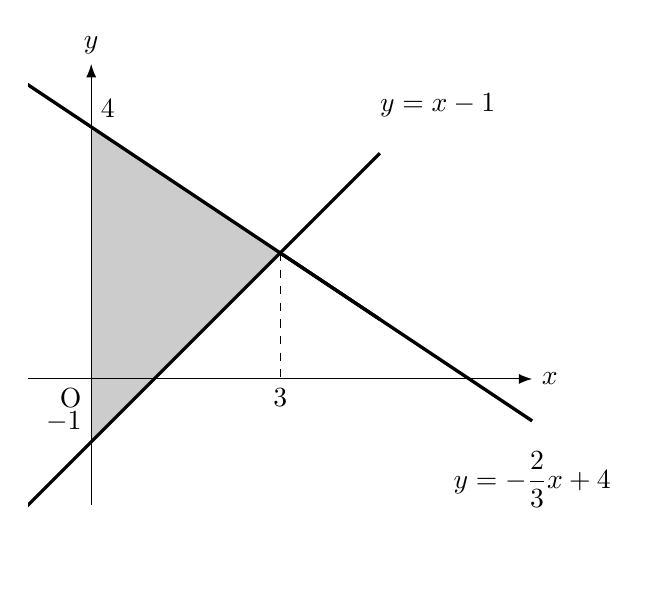
\begin{tikzpicture}[scale=0.8]
    
        \begin{scope}
            \clip(-1,-3)rectangle(7,5);
            \node[below left]at(0,0){O};
            \node[above right]at(0,4){4};
            \node[above left]at(0,-1){$-1$};
            \fill[black!20!white]
            (3,2)
            --plot[domain=3:0](\x,{-2/3*\x+4})
            --(0,-1)
            --plot[domain=0:3](\x,{\x-1})
            --cycle;
            \draw[very thick]plot(\x,{\x-1});
            \draw[very thick]plot(\x,{-2/3*\x+4});
            \draw[dashed](3,2)--(3,0)node[below]{3};
        \end{scope}
        \draw[very thick,domain=3:7]plot(\x,{-2/3*\x+4});
        \node[below]at(7,-1){$y=-\dfrac{2}{3}x+4$};
        \node[above]at(5.5,4){$y=x-1$};
        \draw[->,>=Latex](-1,0)--(7,0)node[right]{$x$};
        \draw[->,>=Latex](0,-2)--(0,5)node[above]{$y$};

    \end{tikzpicture}
\end{center}
上図の網目部$がDで境界をすべて含む.$\\
\kakkonib $-2x+y=kとおいて,下図に図示すると,下図太実線部がy=2x+kである.$
\begin{center}
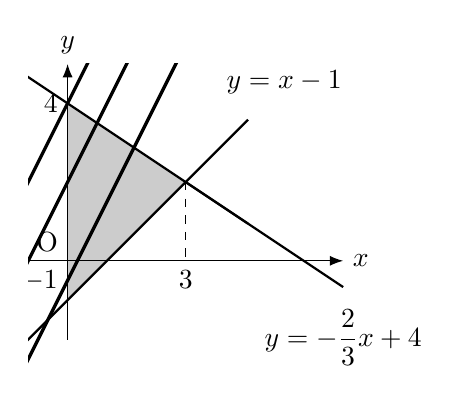
\begin{tikzpicture}[scale=0.5]
        \begin{scope}
            \clip(-1,-3)rectangle(7,5);
            \node[above left]at(0,0){O};
            \node[ left]at(0,4){4};
            \node[above left]at(0,-1){$-1$};
            \fill[black!20!white]
            (3,2)
            --plot[domain=3:0](\x,{-2/3*\x+4})
            --(0,-1)
            --plot[domain=0:3](\x,{\x-1})
            --cycle;
            \draw[thick]plot(\x,{\x-1});
            \draw[thick]plot(\x,{-2/3*\x+4});
            \draw[dashed](3,2)--(3,0)node[below]{3};
            \draw[very thick]plot(\x,{2*\x+4});
            \draw[very thick]plot(\x,{2*\x+2});
            \draw[very thick]plot(\x,{2*\x-1/2});
        \end{scope}
        \draw[thick,domain=3:7]plot(\x,{-2/3*\x+4});
        \node[below]at(7,-1){$y=-\dfrac{2}{3}x+4$};
        \node[above]at(5.5,4){$y=x-1$};
        \draw[->,>=Latex](-1,0)--(7,0)node[right]{$x$};
        \draw[->,>=Latex](0,-2)--(0,5)node[above]{$y$};

    \end{tikzpicture}
\end{center}
$\Y 上図より,(x,y)=(0,4)を通るとき最大より,\\求める最大値は,\kotaee{(x,y)=(0,4)のとき,\max k=4}$
\newpage
\kakkosanb $2x+y=\ell とおいて,下図に図示すると,下図太実線部がy=-2x+\ell である.$
\begin{center}
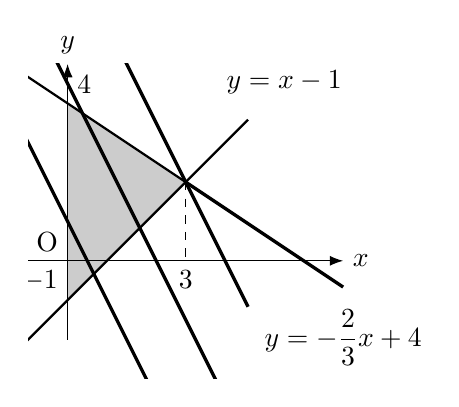
\begin{tikzpicture}[scale=0.5]
    
        \begin{scope}
            \clip(-1,-3)rectangle(7,5);
            \node[above left]at(0,0){O};
            \node[above right]at(0,4){4};
            \node[above left]at(0,-1){$-1$};
            \fill[black!20!white]
            (3,2)
            --plot[domain=3:0](\x,{-2/3*\x+4})
            --(0,-1)
            --plot[domain=0:3](\x,{\x-1})
            --cycle;
            \draw[thick]plot(\x,{\x-1});
            \draw[thick]plot(\x,{-2/3*\x+4});
            \draw[dashed](3,2)--(3,0)node[below]{3};

            \draw[very thick]plot(\x,{-2*\x+1});
            \draw[very thick]plot(\x,{-2*\x+4.5});
            \draw[very thick]plot(\x,{-2*\x+8});
        \end{scope}
        \draw[very thick,domain=3:7]plot(\x,{-2/3*\x+4});
        \node[below]at(7,-1){$y=-\dfrac{2}{3}x+4$};
        \node[above]at(5.5,4){$y=x-1$};
        \draw[->,>=Latex](-1,0)--(7,0)node[right]{$x$};
        \draw[->,>=Latex](0,-2)--(0,5)node[above]{$y$};

    \end{tikzpicture}
\end{center}
$\Y 上図より,(x,y)=(3,2)を通るとき最大より,\\求める最大値は,\kotaee{(x,y)=(3,2)のとき,\max \ell=8}$\\\\
\kakkoshib$ax+y=mとおいて,a=0,a>\dfrac{2}{3},a<\dfrac{2}{3}の三つの場合で分けて考える.$\\
 \underline{\tokeiichi$a=0のとき,$}\\
  $y=mなので,(x,y)=(0,4)のとき,\max m=4である.$\\\\
 \underline{\tokeini$a>\dfrac{2}{3}$のとき,}\\
  $このとき,y=-ax+mは,傾き負の1次関数で,y=-\dfrac{2}{3}x+4の傾きよりも大きくなるので
(x,y)=(0,4)で\max m=4である.$\\\\
 \underline{\tokeisan$a<\dfrac{2}{3}$のとき,}\\
  $ このとき,y=-ax+mは,傾き負の1次関数で,y=-\dfrac{2}{3}x+4の傾きよりも小さくなるので
(x,y)=(3,2)で\max m=2-3aである.$\\
$\Y 以上より,求める最大値は,$
\begin{align*}
    \kotaee{\max m=\begin{cases}
        4   \p{a=0,a>\frac{2}{3}}\\
        2-3a \p{a<\frac{2}{3}}
    \end{cases}}
\end{align*}
\newpage
\noindent\reibanni\\
\noindent\chud 幾何学図形(座標平面に書かないやつ.)を書くには,僕の技量不足で書けないので,あとで別紙(手書き)を渡します.\hiraayamari\\
\kangaekata\\
ベクトルの典型的な問題です.\kakkogob の係数比較の計算が厄介ですがこれも完答をして欲しいところです.\\
\kai\\
\kakkoichib $角の二等分線の性質より,\mathrm{AC:AB=6:5}なので,$
\begin{align*}
    \kotaee{\Vec{OC}=\dfrac{5}{11}\vec{a}+\dfrac{6}{11}\vec{b}}
\end{align*}\\
\kakkonib 添付図のように点$\mathrm{D,E}をおく.このとき,p,q\in\mathbb{R}に対して,$
\begin{align*}
    \begin{cases}
        \mathrm{EI:IB=p:1-p}\\
        \mathrm{DI:IA=q:1-q}
    \end{cases}
\end{align*}
とおくと,
\begin{align*}
    \begin{cases}
    \Vec{OI}=p\vec{b}+\frac{5}{12}(1-p)\vec{a}\cdots\cdots\cdots\maruichi\\
    \Vec{OI}=q\vec{a}+\frac{6}{13}(1-q)\vec{b}\cdots\cdots\cdots\maruni
        \end{cases}
\end{align*}
$\maruichi,\maruni $をそれぞれ係数比較して,
\begin{align*}
    \begin{cases}
    p=\frac{6}{13}(1-q)\\
    \frac{5}{12}(1-p)=q
    \end{cases}&\doti \begin{cases}
        13p=6\p{1-\frac{5}{12}+\frac{5}{12}p}\\
        q=\frac{5}{12}(1-p)
    \end{cases}\\
    &\doti\begin{cases}
        p=\frac{1}{3}\\
        q=\frac{5}{18}
    \end{cases}
\end{align*}
$\Y \kotaee{\Vec{OI}=\dfrac{5}{18}\vec{a}+\dfrac{1}{3}\vec{b}}$\\\\
\kakkosanb 余弦定理より,
\begin{align*}
    \cos\Kaku{BOA}=\dfrac{25+36-49}{2\cdot5\cdot6}=\dfrac{1}{6}
\end{align*}
なので,
\begin{align*}
    \vec{a}\cdot\vec{b}=\kotaee{6}
\end{align*}
\newpage
\noindent\kakkoshib 添付の図より,
\begin{align*}
    \Vec{AH}&=\Vec{OH}-\vec{a}\\
    &=\kotaee{(s-1)\vec{a}+t\vec{b}}
\end{align*}
同様にして,
\begin{align*}
    \Vec{BH}&=\Vec{OH}-\vec{b}\\
    &=\kotaee{s\vec{a}+(t-1)\vec{b}}
\end{align*}\\
\kakkogob 重心の性質より,
\begin{align*}
    \begin{cases}
        \Vec{AH}\cdot\vec{b}=0\\
        \Vec{BH}\cdot\vec{a}=0
    \end{cases}&\doti\begin{cases}
        (s-1)\vec{a}\cdot\vec{b}+t\left|\vec{b}\right|^2=0\\
        s\left|\vec{a}\right|^2+(t-1)\vec{a}\cdot\vec{b}=0
    \end{cases}\\
    &\doti\begin{cases}
        6s+25t=6\\
        6s+t=1
    \end{cases}\\
    &\doti\begin{cases}
        t=\frac{5}{24}\\
        6s=\frac{9}{24}
    \end{cases}\\
    &\doti\kotaee{\begin{cases}
        s=\frac{9}{144}\\
        t=\frac{5}{24}
    \end{cases}}
\end{align*}
\newpage
\noindent\reibansan\\
\kangaekata 数列は集合論で定義されている問題です.抽象的な数学(大学数学とか)に慣れていないと解答できる問題は,1つもないのではないでしょうか.
これは全滅でも仕方ありません.\\
\kai\\
$n\in\mathbb{N}\geq3.S=\B{a_1,a_2,\cdots,a_n}.a_1=k$\\
\kakkoichib,\kakkonib $a_i-a_1(i\geq2)\in Sのとき,a_2を求める.$
\begin{align*}
    &a_1\\
    &a_2-k\\
    &a_3-k\\
    &a_4-k\\
    &\vdots\\
    &a_n-k
\end{align*}
は$すべてSの元になるので,a_n-k<a_nより,S=\B{a_2-k,a_3-k,\cdots,a_n-k}について,これは等差数列になる.$\\
すなわち,
\begin{align*}
    &a_2-k=a_2-a_1=k\narabaa a_2=2k\\
    &a_3-k=a_3-a_1=(a_2+k)-k\narabaa a_3=3k\\
    &\vdots\\
    &a_n=nk
\end{align*}
$\Y \kotaee{a_2=2k} \kakkoichib$\\
$\Y \kotaee{a_n=nk} \kakkonib$\\\\
\kakkosanb $\dfrac{a_i}{a_1}(i\geq2)がすべてSの元のとき,\B{\dfrac{a_i}{k}}は$
\begin{align*}
    {\dfrac{a_2}{k},\dfrac{a_3}{k},\cdots,\dfrac{a_n}{k}}\cdots\cdots\cdots\asta 
\end{align*}
なので,$kが次の3つの場合のときを考える.$
\begin{align*}
    \begin{cases}
        k=1\\
        0<k<1\\
        k>1
    \end{cases}
\end{align*}
 \noindent\underline{\tokeiichi $k=1のとき$}\\
  $このとき\asta は,$
\begin{align*}
    \B{a_2,a_3,\cdots,a_n}
\end{align*}
となるので,$a_nはnで表すことができない.$\\\\
\underline{\tokeini $0<k<1のとき$}\\
  $このとき,すべてのiに対して,\dfrac{a_i}{k}>a_nになるので,下限から上限までのすべての元がSの元にならない.\\
  よって,a_nは存在しない.$\\\\
 \underline{\tokeisan$k>1$のとき}\\
  $このとき,すべてのiに対して,\dfrac{a_i}{k}<a_nになるので,確かにSの元になる.$\\
従って,
\begin{align*}
    &\dfrac{a_2}{k}=\dfrac{a_2}{a_1}=\dfrac{a_1\cdot k}{a_1}=k\narabaa a_2=k^2\\
    &\dfrac{a_3}{k}=\dfrac{a_3}{a_1}=\dfrac{a_2\cdot k}{a_1}=k^2\narabaa a_3=k^3\\
    &\vdots\\
    &\dfrac{a_n}{k}=k^{n-1}\narabaa a_n=k^n
\end{align*}
$\Y a_n=k^n.$\\
$\Y 以上より,a_nは$
\begin{align*}
    \kotaee{a_n=\begin{cases}
        表せない.(k>1)\\
        存在しない.(0<k<1)\\
        k^n(k>1)
    \end{cases}}
\end{align*}
\newpage
\subsection{2025年度実施}
\reibanichi\\
\kangaekata\\
剰余に関する問題です.$n桁の数の1の位の数を調べたかったら,\ans{\mod10 で考える.}というのが鉄則です.$\\
\kai\\
\kakkoichib $f_2(n)\doti n^2の1の位.$\\
$以下,\mod10で考える.$
\begin{center}
    \begin{tabular}{|c||c|c|c|c|c|c|c|c|c|}
        \hline
        $n$ & $1$ & $2$ & $3$ & $4$ & $5$ & $6$ & $7$ & $8$ & $9$ \\
        \hline
        $n^2$ & $1$ & $4$ & $9$ & $16$& $25$ & $36$&  $49$ & $64$ & $81$ \\
        \hline
        $n^2\kmod{10}$& $1$ & $4$&  $9$&  $6$ & $5$ & $6$ & $9$ & $4$ & $1$ \\
        \hline
    \end{tabular}
\end{center}
$上表より,f_2(n)は,0,1,4,5,6,9を周期的に繰り返し,その周期は6である.$\\
$\Y \kotaee{0,1,4,5,6,9}$\\\\
\kakkonib $f_5(n)-f_1(n)\doti n^5-nの1の位$
\begin{center}
    \begin{tabular}{|c||c|c|c|c|c|c|}
        \hline
        $n^2\kmod{10}$ & $0$ &  $1$ & $4$&  $5$&  $6$&  $9$\\
        \hline
        $n^5\kmod{10}$ & $0$ &  $1$ & $4$&  $5$&  $6$&  $9$\\
        \hline
        $n^5-n\kmod{10}$ & $0$ & $0$ & $0$ & $0$ & $0$ & $0$\\
        \hline
    \end{tabular}
\end{center}
$\Y 上表より,f_5(n)-f_1(n)\kotaee{0}$\\\\
\kakkosanb $\kakkonib より,n^5\godo n\kmod{10}なので,$
\begin{align*}
    n^{100}=\p{n^5}^{20}\godo n^20=\p{n^5}^4\godo n^4\kmod{10}
\end{align*}
これより,$n^{100}\godo n^4\kmod{10}$なので,
\begin{center}
    \begin{tabular}{|c||c|c|c|c|c|c|c|c|c|c|}
        \hline
        $n$ & $0$ &$1$& $2$& $3$& $4$& $5$& $6$& $7$ &$8$& $9$\\
        \hline
        $n^4\kmod{10}$ & $0$ & $1$ & $6$ & $1$ & $6$ & $5$ & $6$ & $1$ & $6$ & $1$\\
        \hline 
    \end{tabular}
\end{center}
これよ,$0,1,5,6を周期的に繰り返すので,\kotaee{0,1,5,6}$
\newpage
\reibanni\\
\kangaekata\\
階差数列に関する問題です.これは完答しましょう.\\
\kai\\
\kakkoichib $b_n=\kotaee{-\dfrac{1}{n+1}+\dfrac{1}{n}}$\\\\
\kakkonib \begin{align*}
    a_n&=a_1+\wa{k=1}{n-1}\B{\dfrac{1}{k}-\dfrac{1}{k+1}}\\
    &=a_1-\wa{k=1}{n-1}\B{\dfrac{1}{k+1}-\dfrac{1}{k}}\\
    &=1-\tint{\dfrac{1}{n}}{1}{n}\\
    &=2-\dfrac{1}{n} (n\geq2)
\end{align*}
$また,これはn=1のときも成立している.\\
\Y \kotaee{a_n=2-\dfrac{1}{n}}$\\\\
\kakkosanb $\Delta a_n=n(n+1)なので,和差分の関係より,$
\begin{align*}
    a_n&=\wa{k=1}{n-1}\Delta a_n\\
    &=\tint{\dfrac{1}{3}n(n-1)(n+1)}{1}{n}\\
    &=\kotaee{\dfrac{1}{3}(n-1)n(n+1)}
\end{align*}
\newpage
\noindent\reibansan\\
\kangaekata\\
$三角関数と解の個数の問題です.この種の問題で一番難しいと思いました.特に,\kakkosanb では,\ans{対応するkの個数と\theta の個数}に注意しないといけません.$\\
\kai\\
\kakkoichib\begin{align*}
    f(\theta)&=2\cos^2\theta-1-2\sqrt{3}\sin\theta\cos\theta+2\cdot2\cos\frac{\theta}{2}\sin\frac{\theta}{2}-4\sqrt{3}\cos^2\frac{\theta}{2}+2\sqrt{3}\\
    &=2\cos^2\theta-2\sqrt{3}\sin\theta\cos\theta+2\sin\theta-4\sqrt{3}\cdot\dfrac{1+\cos\theta}{2}+2\sqrt{3}\\
    &=2\cos^2\theta-2\sqrt{3}\sin\theta\cos\theta+2\sin\theta-2\sqrt{3}-2\sqrt{3}\cos\theta+2\sqrt{3}-1\\
    &=\p{2\cos^2\theta-2\sqrt{3}\sin\theta\cos\theta+1}-2+2\p{\sin\theta-\sqrt{3}\cos\theta}\cdots\cdots\cdots\maruichi 
\end{align*}
また,$k^2=2\cos^2\theta-2\sqrt{3}\sin\theta\cos\theta+1なので,\maruichi について,$
\begin{align*}
    f(\theta)=\kotaee{k^2+2k-2}
\end{align*}\\
\kakkonib $ここで,g(k)=k^2+2k-2とおく.$\\
$k=2\sin\p{\theta-\dfrac{\pi}{3}}なので,kの取りうる値の範囲は,-\dfrac{\pi}{3}\leq\theta-\dfrac{\pi}{3}\leq\dfrac{2\pi}{3}\cdots\cdots\cdots\asta である.\\
このことより,$
\begin{align*}
    -\dfrac{\sqrt{3}}{2}\leq\sin\p{\theta-\dfrac{\pi}{3}}\leq1\doti -\sqrt{3}\leq k\leq 2
\end{align*}

    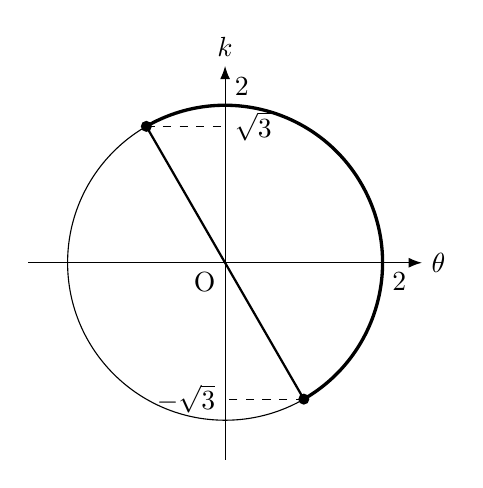
\begin{tikzpicture}
        \draw[->,>=Latex](-2.5,0)--(2.5,0)node[right]{$\theta$};
        \draw[->,>=Latex](0,-2.5)--(0,2.5)node[above]{$k$};
        \draw(0,0)circle[radius=2];
        \draw[very thick]({2*cos(-60)},{2*sin(-60)})
    arc[start angle=-60, end angle=120, radius=2];
    \fill(-1,{sqrt(3)})circle(2pt);
    \fill(1,{-sqrt(3)})circle(2pt);
    \draw[thick](-1,{sqrt(3)})--(1,{-sqrt(3)});
    \node[below left]at(0,0){O};
    \node[above right]at(0,2){2};
    \draw[dashed](-1,{sqrt(3)})--(0,{sqrt(3)})node[ right]{$\sqrt{3}$};
    \draw[dashed](1,{-sqrt(3)})--(0,{-sqrt(3)})node[left]{$-\sqrt{3}$};
    \node[below right]at(2,0){2};
    \end{tikzpicture}
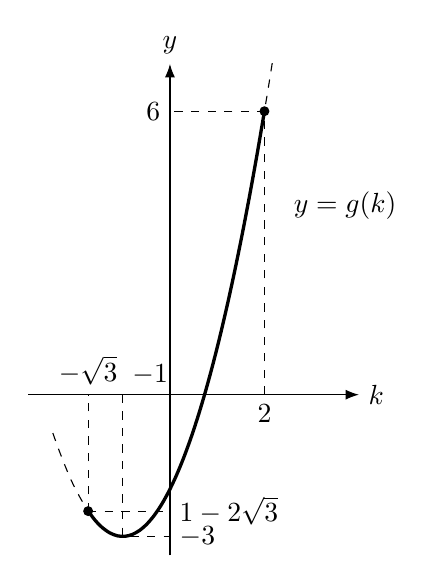
\begin{tikzpicture}[scale=0.6]
     \draw[->,>=Latex](-3,0)--(4,0)node[right]{$k$};
    \draw[->,>=Latex](0,-3.4)--(0,7)node[above]{$y$};
    \begin{scope}
       \clip (-2.5,-3.2)rectangle(3,7);
       \draw[dashed,smooth]plot(\x,{pow(\x,2)+2*\x-2});
       \draw[very thick,smooth,domain={-sqrt(3)}:2]plot(\x,{pow(\x,2)+2*\x-2});
       \fill({-sqrt(3)},{1-2*sqrt(3)})circle(3pt);
       \draw[dashed]({-sqrt(3)},{1-2*sqrt(3)})--(0,{1-2*sqrt(3)})node[right]{$1-2\sqrt{3}$};
       \draw[dashed]({-sqrt(3)},{1-2*sqrt(3)})--({-sqrt(3)},0)node[above]{$-\sqrt{3}$};
       \draw[dashed](-1,0)--(-1,-3)--(0,-3)node[right]{$-3$};
       \node[above right]at(-1,0){$-1$};
       \fill(2,6)circle(3pt);
       \draw[dashed](2,0)--(2,6)--(0,6)node[left]{$6$};
       \node[below]at(2,0){2};
 \end{scope}
           \node[left]at(5,4){$y=g(k)$};
\end{tikzpicture}
\newpage
\noindent 上図より,$y=g(k)はk=-1を対称軸とする下に凸の放物線なので,求める最大値及び最小値は,$
\begin{align*}
    &k=-1\doti \theta=\dfrac{\pi}{6}のとき,最大値を取る.\\
    &k=2\doti \theta=\dfrac{5\pi}{6}のとき,最小値を取る.
\end{align*}
$\Y 求める最大値及び最小値は,$
\begin{align*}
    \kotaee{\begin{cases}
        \max g(k)=6 \p{\theta=\frac{5\pi}{6}}\\
        \min g(k)=-3 \p{\theta=\frac{\pi}{6}}
    \end{cases}}
\end{align*}\\
\kakkosanb \begin{align*}
    &\kakkoichi のkに対して,f(\theta)=ak の解の個数を求める.\\
    &\doti f(\theta)=akの共有点の個数は,ky平面における(k,y)の個数に対応する.(全射であって,単射ではない.)\\
    &また,その(k,y)に対して,\theta k平面の共有点(\theta,k)に変換したものが求める解の個数.(これも全射)
\end{align*}
以下,\chud\\
上で言っていることはすなわち,\\
$\ans{y=g(k)とy=akの共有点の個数は本来求める解の個数ではない.}\\
\ans{y=f(\theta)とy=akの共有点の個数が本来求めるもの.}ということ.$イメージは下みたいな感じ.
\begin{center}
    「$y=g(k)とy=akの共有点の個数$ (\kakkoni の放物線の座標平面で考える)」\\$\xrightarrow{変換}$ 「$y=f(\theta)とy=akの共有点の個数$ (\kakkoni の円の座標平面で考える)」\ans{\chud 終わり}
\end{center}
\begin{center}
    \begin{tikzpicture}[scale=1.5]
    \draw[->,>=Latex](-2.5,0)--(2.5,0)node[right]{$\theta$};
    \draw[->,>=Latex](0,-2.5)--(0,2.5)node[above]{$k$};
    \draw(0,0)circle[radius=2];
    \draw[very thick]({2*cos(-60)},{2*sin(-60)})
    arc[start angle=-60, end angle=120, radius=2];
    \fill(-1,{sqrt(3)})circle(2pt);
    \fill(1,{-sqrt(3)})circle(2pt);
    \draw[thick](-1,{sqrt(3)})--(1,{-sqrt(3)});
    \node[below left]at(0,0){O};
    \node[above right]at(0,2){2};
    \draw[dashed](-1,{sqrt(3)})--(2.2,{sqrt(3)})node[right]{$\sqrt{3}$};
    \draw[dashed](0,{-sqrt(3)})--(2.2,{-sqrt(3)})node[right]{$-\sqrt{3}$};
   \draw[<->,>=Latex](2.1,{-sqrt(3)})--(2.1,{sqrt(3)});
   \node[right]at(2.1,1){$\theta は1個定まる.(-\sqrt{3}\leq k<\sqrt{3},k=2)$};
   \draw[dashed](-1,{sqrt(3)})--(-2.2,{sqrt(3)});
   \draw[dashed](0,2)--(-2.2,2);
   \draw[<->,>=Latex](-2.1,2)--(-2.1,{sqrt(3)});
   \node[left]at(-2.3,{sqrt(3)+0.2}){$\theta は2個定まる.(\sqrt{3}\leq k<2)$};
    \node[below right]at(2,0){2};
    \end{tikzpicture}
\end{center}
\newpage
P.50の図より,$-\sqrt{3}\leq k<\sqrt{3},k=2のとき\theta は1つ決まり,\sqrt{3}\leq k<2のとき\theta は2つ決まる.$\\
このことから,$k=-\sqrt{3},-1,\sqrt{3},2上の放物線の座標を通る直線を描くと下図を得る.$
\begin{center}
    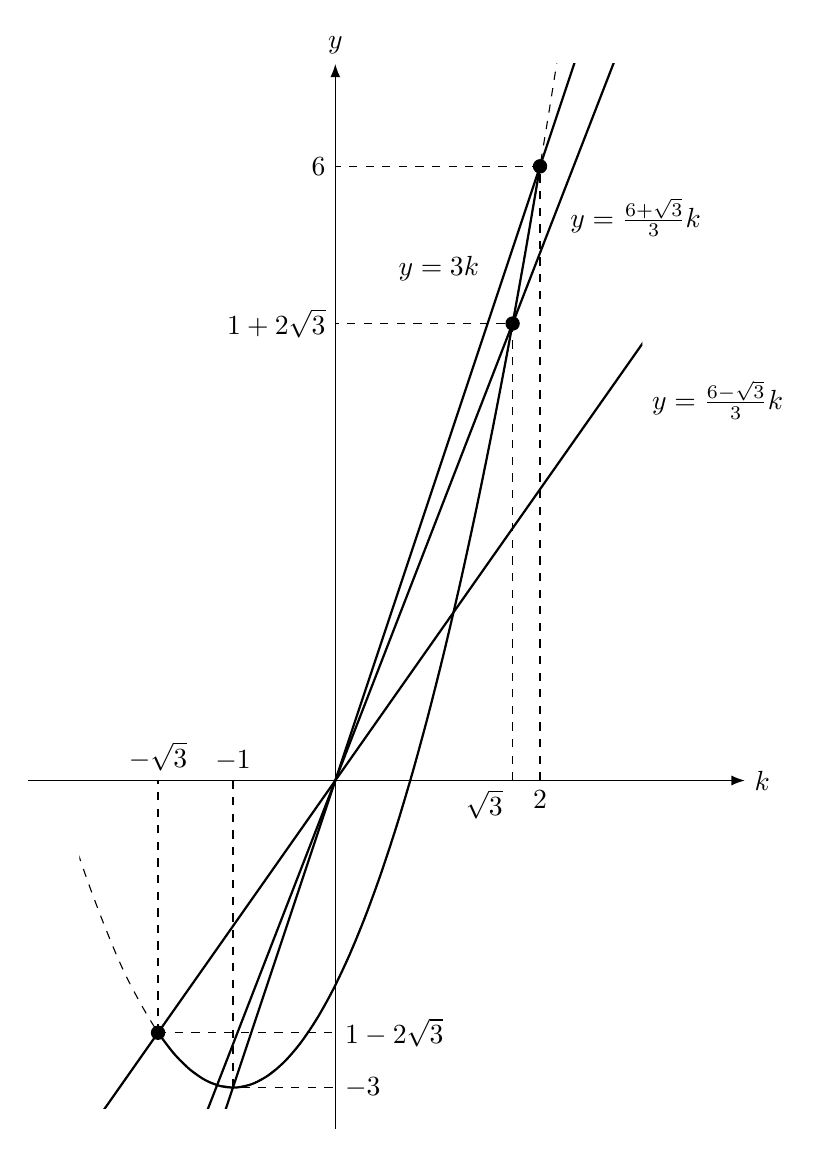
\begin{tikzpicture}[scale=1.3]
     \draw[->,>=Latex](-3,0)--(4,0)node[right]{$k$};
    \draw[->,>=Latex](0,-3.4)--(0,7)node[above]{$y$};
    \begin{scope}
       \clip (-2.5,-3.2)rectangle(3,7);
       \draw[dashed,smooth]plot(\x,{pow(\x,2)+2*\x-2});
       \draw[ thick,smooth,domain={-sqrt(3)}:2]plot(\x,{pow(\x,2)+2*\x-2});
       \fill({-sqrt(3)},{1-2*sqrt(3)})circle(2pt);
       \draw[dashed]({-sqrt(3)},{1-2*sqrt(3)})--(0,{1-2*sqrt(3)})node[right]{$1-2\sqrt{3}$};
       \draw[dashed]({-sqrt(3)},{1-2*sqrt(3)})--({-sqrt(3)},0)node[above]{$-\sqrt{3}$};
       \draw[dashed](-1,0)--(-1,-3)--(0,-3)node[right]{$-3$};
       \node[above]at(-1,0){$-1$};
       \fill(2,6)circle(2pt);
       \draw[dashed](2,0)--(2,6)--(0,6)node[left]{$6$};
       \node[below]at(2,0){2};
       \draw[dashed]({sqrt(3)},0)--({sqrt(3)},{1+2*sqrt(3)})--(0,{1+2*sqrt(3)})node[left]{$1+2\sqrt{3}$};
       \draw[thick]plot(\x,{2*\x-sqrt(3)/3*\x});
       \draw[thick]plot(\x,{3*\x});
       \draw[thick]plot(\x,{2*\x+sqrt(3)/3*\x});
       \fill({sqrt(3)},{1+2*sqrt(3)})circle(2pt);
       \node[below left]at({sqrt(3)},0){$\sqrt{3}$};


 \end{scope}
      \node[below right]at(3,4){$y=\frac{6-\sqrt{3}}{3}k$}; 
      \node[left]at(1.5,5){$y=3k$};    
      \node[right]at(2.2,5.5){$y=\frac{6+\sqrt{3}}{3}k$};
 
\end{tikzpicture}
\end{center}
上図より,\\
   $\bullet 0<a<\dfrac{6-\sqrt{3}}{3} のとき,kは1つで,対応する\theta は\mathrm{P.50}の図でk>0側に1つ.\\
    \bullet \dfrac{6-\sqrt{3}}{3}\leq a<\dfrac{6+\sqrt{3}}{3}のとき,kは2つで,-\sqrt{3}\leq k<\sqrt{3}より対応する\theta は\mathrm{P.50}の図でk>0側に1つ,k<0側に1つで合計2つ.\\
    \bullet \dfrac{6+\sqrt{3}}{3}\leq a<3のとき,kは2つで,\sqrt{3}\leq k<2より対応する\theta は\mathrm{P.50}の図でk>0側に2つ,k<0側に1つで合計3つ.\\
    \bullet a=3のとき,kは2つで,k=2より対応する\theta は2つ.$
まとめると次のようになる.
\newpage
\noindent
\begin{align*}
    \kotaee{\begin{cases}
        0<a<\dfrac{6-\sqrt{3}}{3} のとき,対応する\theta は1つ.\\
        \dfrac{6-\sqrt{3}}{3}\leq a<\dfrac{6+\sqrt{3}}{3},a=3のとき,対応する\theta は2つ.\\
        \dfrac{6+\sqrt{3}}{3}\leq a<3のとき,対応する\theta は3つ.
    \end{cases}}
\end{align*}
\newpage
\section{良問集解答編}
\subsection{第1回}
\ba{1.0}\\
\kai\\
\kakkoichib  両辺が0以上であるから,両辺2乗しても同値性は崩れないので,両辺を2乗することにより,
\begin{align*}
    (x+3)^2\geq(x-2)^2&\doti x^2+6x+9\geq x^2-4x+4\\
    &\doti\kotaee{x\geq-\dfrac{1}{2}}
\end{align*}\\
\kakkonib  両辺が0以上であるから,両辺2乗しても同値性は崩れないので,両辺を2乗することにより,
\begin{align*}
    (4x-1)^2<(x+3)^2&\doti (4x-1)^2-(x+3)^2<0\\
    &\doti \B{(4x-1)+(x+3)}\B{(4x-1)-(x+3)}<0\\
    &\doti (5x+2)(3x-4)<0\\
    &\doti\kotaee{-\dfrac{2}{5}<x<\dfrac{4}{3}}
\end{align*}\\\\
\fbox{\kurosankakub 類題演習1.1\kurosankakua}\\
\kai\\
\kakkoichib \begin{align*}
    |2x-3|\leq2&\doti -2\leq2x-3\leq2\\
    &\doti \kotaee{\dfrac{1}{2}\leq x\leq\dfrac{5}{2}}
\end{align*}
また,$|2x-3|\leq2\leq\dfrac{1-3a}{3}x-1は,-\dfrac{2}{5}<x<\dfrac{4}{3}かつ\dfrac{1-3a}{3}x\geq3\cdots\cdots\maruichi 
となり\maruichi がx\geq1 のとき,1\leq x\leq\dfrac{5}{2}を得る.\\ 
従って,1-3a>1のとき,x\geq\dfrac{9}{1-3a}.この式の右辺が\dfrac{9}{1-3a}=1となるのは,\kotaee{a=-\dfrac{8}{3}}である.$
\newpage
\noindent\kakkonib\begin{align*}
    |x|+|x-3|<4&\doti |x|<4-|x-3|\\
    &\doti |x-3|-4<x<4-|x-3|\\
    &\doti\begin{cases}
        |x-3|<x+4\\
        |x-3|<4-x
    \end{cases}\\
    &\doti\begin{cases}
        -(x+4)<x-3<x+4\\
        x-4<x-3<-x+4
    \end{cases}\\
    &\doti\begin{cases}
        x>-\frac{1}{2}\\
        x<\frac{7}{2}
    \end{cases}\\
    &\doti\kotaee{-\dfrac{1}{2}<x<\dfrac{7}{3}}
\end{align*}\\\\
\ba{1.2.0}\\
\kai\\
与えられた状況を図示すると下図のようになる.
\begin{center}
    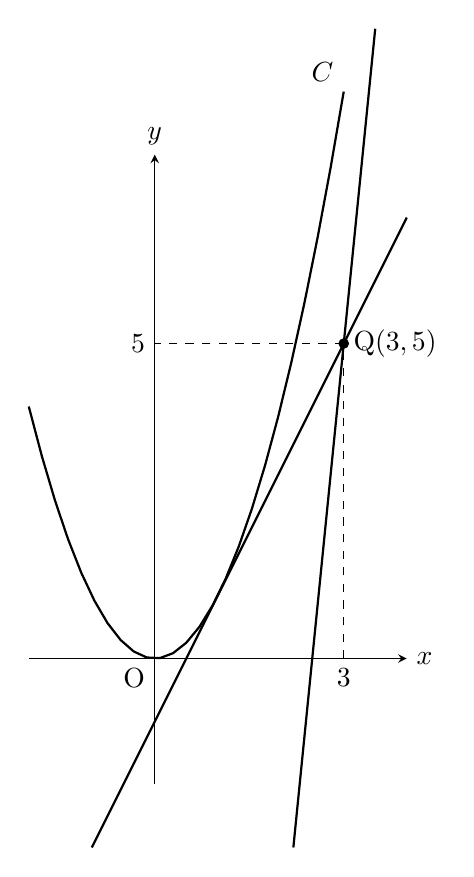
\begin{tikzpicture}[scale=0.8]
        \draw[->,>=stealth](-2,0)--(4,0)node[right]{$x$};
        \draw[->,>=stealth](0,-2)--(0,8)node[above]{$y$};
        \draw[thick,domain=-2:3]plot(\x,{pow(\x,2)})node[above left]{$C$};
        \draw[thick,domain=-1:4]plot(\x,{2*\x-1});
        \draw[thick,domain=2.2:3.5]plot(\x,{10*\x-25});
        \draw[dashed](3,0)--(3,5)--(0,5)node[left]{5};
        \node[below]at(3,0){3};
        \node[right]at(3,5){Q$(3,5)$};
        \fill(3,5)circle(2.4pt);
        \node[below left]at(0,0){O};
    \end{tikzpicture}
\end{center}
\newpage
\noindent\kakkoichib $2本の接線とy=x^2の接点のx座標をx=sとおくと,この点における接線の方程式は,$
\begin{align*}
    y=2s(x-s)+s^2\cdots\cdots\cdots\maruichi
\end{align*}
$\maruichi が点\mathrm{Q}(3,5)を通るので,$
\begin{align*}
    5=2s(3-s)+s^2&\doti -s^2+6s=5\\
    &\doti (s-1)(s-5)=0
\end{align*}
$\Y s=1,5$\\
$\Y s=1のとき,\maruichi:y=2(x-1)+1 \Y \kotaee{y=2x-1,接点(1,1)}\\
    s=5のとき,\maruichi:y=10(x-5)+25\Y \kotaee{y=10x-25,接点(5,25)}$\\\\
\kakkonib $\mathrm{P}が(2,4)から(-3,9)まで動くとき,線分\mathrm{PQ}が通過する領域は,下図の網目部である.$
\begin{center}
    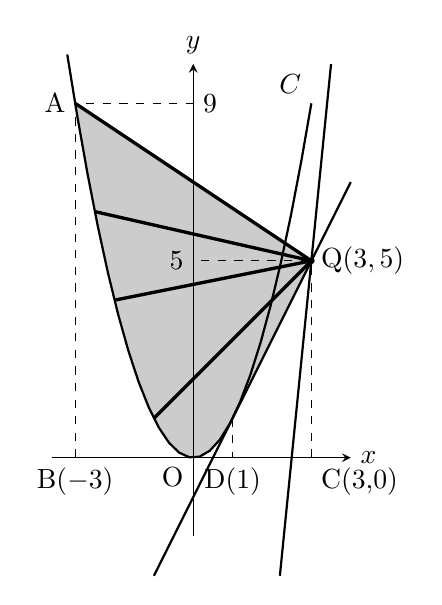
\begin{tikzpicture}[scale=0.5]
        \draw[->,>=stealth](-3.6,0)--(4,0)node[right]{$x$};
        
        \fill[black!20!white]plot[domain=-3:1](\x,{pow(\x,2)});
        
        \filldraw[black!20!white](-3,9)--(1,1)--(3,5)--(-3,9)--cycle;
        \draw[->,>=stealth](0,-2)--(0,10)node[above]{$y$};
        \draw[thick,domain=-3.2:3]plot(\x,{pow(\x,2)})node[above left]{$C$};
        \draw[thick,domain=-1:4]plot(\x,{2*\x-1});
        \draw[thick,domain=2.2:3.5]plot(\x,{10*\x-25});
        \draw[dashed](3,0)--(3,5)--(0,5)node[left]{5};
        \node[below right]at(3,0){C(3,0)};
        \node[right]at(3,5){Q$(3,5)$};
        \fill(3,5)circle(2.4pt);
        \node[below left]at(0,0){O};
        \draw[dashed](-3,0)--(-3,9)--(0,9)node[right]{9};
        \draw[dashed](1,1)--(1,0)node[below]{D(1)};
        \node[below]at(-3,0){B$(-3)$};
        \draw[very thick](3,5)--(-3,9);
        \draw[very thick](3,5)--(-2,4);
        \draw[very thick](3,5)--(-1,1);
        \draw[very thick](3,5)--(-2.5,6.25);
        \node[left]at(-3,9){A};
    \end{tikzpicture}
\end{center}
ここで,$(-3,9)を\mathrm{A},(-3,0)を\mathrm{B},(3,0)を\mathrm{C},(1,0)を\mathrm{D},(1,1)を\mathrm{E}とすると,求める面積Sは,$
\begin{align*}
    S&=(台形\mathrm{ABCQ})-\p{\dint{-3}{1}x^2dx+台形(\mathrm{DEQB})}\\
    &=\dfrac{1}{2}(9+5)\cdot6-\p{\dfrac{1}{3}\tint{x^3}{-3}{1}-\dfrac{1}{2}(1+5)\cdot2}\\
    &=36-\dfrac{28}{3}\\
    &=\kotaee{\dfrac{80}{3}}
\end{align*}
\newpage
\noindent\ba{1.2.1}\\
\kai\\
まずは,図示すると下図のような状況.
\begin{center}
    \begin{tikzpicture}[scale=0.3]
        \draw[->,>=stealth](-2,0)--(30,0)node[right]{$x$};
        \draw[->,>=stealth](0,-2)--(0,25)node[above]{$y$};
        \draw[thick,domain=0:25]plot(\x,{-0.8*\x+20});
        \node[left]at(0,20){B:20};
        \node[below]at(25,0){A:25};
        \fill(0,20)circle(10pt);
        \fill(25,0)circle(10pt);
        \draw[thick](10,0)circle[radius=6];
        \node[below]at(10,0){C:10};
        \fill(10,0)circle(10pt);
        \node[below left]at(0,0){O};
        \coordinate(A)at(25,0);
        \coordinate(B)at(0,20);
        \coordinate(C)at(10,0);
        \draw[thick] (C) --($(A)!(C)!(B)$)node[above right]{H};
        \coordinate(H)at($(A)!(C)!(B)$);
        \pic[draw,angle radius=2mm]{right angle=C--H--A};
        \node[below ]at(13.75,4.65){$\mathrm{P_0}$};
        \fill(13.75,4.65)circle(10pt);
        \draw[thick](B)--(13.75,4.65)--(A);
    \end{tikzpicture}
\end{center}
ここで,線分ABにCから引いた垂線の足をH,HからCに向かって引いた直線と円との交点を$\mathrm{P_0}とすると,円上を動く\mathrm{P}が
\mathrm{P_0}にきた時に\Sankaku{ABP}は最小になるので,$
\begin{align*}
    \Sankaku{ABP}=\dfrac{1}{2}\cdot\mathrm{AB}\cdot(\mathrm{AH}-6)\cdots\cdots\cdots\maruichi
\end{align*}
と書ける.\\
$ここで,\mathrm{AB}^2=25^2+20^2であり,\mathrm{AB}を通る直線の方程式は,4x+5y=100なので,点と直線の距離公式より,\mathrm{CH}=\dfrac{|4\cdot10-100|}{\sqrt{4^2+5^2}}=\dfrac{60}{\sqrt{4^2+5^2}}.$\\
$\Y \Sankaku{ABP}=\dfrac{1}{2}\cdot5\sqrt{5^2+4^2}\p{\dfrac{10}{\sqrt{5^2+4^2}}-1}6=\kotaee{15\p{10-\sqrt{41}}}$
\newpage
\fbox{\kurosankakub 類題演習1.2.2\kurosankakua}\\
\kai\\
\kakkoichib $O_2の中心がC,半径が2であることより,Cの座標は(1,0)であるとすぐにわかる.$\\
従って3つの円をすべて図示すると下図のようになる.
\begin{center}
  \begin{tikzpicture}[scale=1.3]
\draw[->,>=stealth](0,0)--(5,0)node[right]{$x$};
\draw[->,>=stealth](0,-1)--(0,5)node[above]{$y$};
\begin{scope} \clip (0,0) rectangle (4,4);
  \draw(0,0)circle[radius=3];
  \draw(1,0)circle[radius=2];
  \draw(2.09,1.86)circle[radius=0.175];
\end{scope}
\node[below]at(1,0){1};
\node[right]at(3,0){3};
\fill(1,0)circle(1.5pt);
  \end{tikzpicture}
\end{center}
$よって,\Vec{OC}=\tvec<0,1>[1,0],\Vec{OB}=\tvec<0,1>[2,\sqrt{3}]なので,$
\begin{align*}
  \Vec{CP}&=t\Vec{CB}\\
  &\doti \Vec{OP}=\Vec{OC}+t\Vec{CB}\\
  &\doti \Vec{OP}=\tvec<0,1>[1,0]+t\tvec<0,1>[2,\sqrt{3}]\\
  &\doti \Vec{OP}=\tvec<0,1>[t+1,\sqrt{3}t]
\end{align*}
$\Y \kotaee{\mathrm{P}(t+1,\sqrt{3})}$
\newpage
\noindent\kakkonib $O_3の半径rとすると,\Vec{CP}=t\Vec{CB}より,$
\begin{align*}
  \mathrm{CB}:\mathrm{CP}=1:t
\end{align*}
これより,$\mathrm{BP}=t-1より,r=(t-1)\left|\Vec{CB}\right|=2(t-1).\\
従って,\Vec{OP}=\tvec<0,1>[t+1,\sqrt{3}t]をrを用いて表すと,$
\begin{align*}
  \left|\Vec{OP}\right|=(3-r)=\B{3-2(t-1)}
\end{align*}
このことより,
\begin{align*}
\left|\Vec{OP}\right|^2=(5-2t)^2&\doti (t+1)^2+3t^2=25-20t+4t^2\\
&\doti 22t=24\\
&\doti t=\dfrac{12}{11}
\end{align*}
$\Y \mathrm{P}の座標は,\kotaee{\mathrm{P}\p{\dfrac{23}{11},\dfrac{12\sqrt{3}}{11}}}\\\\
半径rは,r=2\cdot\dfrac{1}{11}=\kotaee{\dfrac{2}{11}}$
\newpage
\subsection{第2回}
\noindent\kangaekata\\
領域・軌跡の総合的な演習です.領域・軌跡の典型的な解答は,\ans{自然流(順像法)}か\ans{逆手流(逆像法)}の2つです.\\
軽くまとめておきましょう.
\begin{itembox}
    [l]{\kagil 軌跡・領域の城跡\kagir}
$y=f(t)のtが全ての実数を動くとき,その軌跡(領域)Wを求めたい.\\
 \doichib \ans{順像法:tをすべての実数で動かして,それらをすべて集める.}\\
 \donib\ans{逆像法:(x,y)\in W\doti y=f(t)を満たすtが少なくとも一つ存在する.\doti\cdots}$
\end{itembox}
\chu 逆像法を選択するか順像法を選択するかは,問題によって違う.例えば,ベクトルの和の形で表すことができるなら,それは順像法のほうが楽な場合が多いです.\\
\ba{2.1.0}\\
\kai\\
$以下,\kakkoichib,\kakkonib,\kakkosanb,\kakkoshib の通過領域をW_i(i=1,2,3,4)とおく.$\\
\kakkoichib \begin{align*}
    (x,y)\in W_1&\doti \exists m>0,m^2-mx+y=0\cdots\cdots\cdots\maruichi
\end{align*}
$ここで,f(m)=m^2-mx+y とおくと,$
\begin{align*}
    \maruichi&\doti \begin{cases}
        x^2-4y\geq0\\
        f(0)>0かつx>0\\
        f(0)<0かつ(x<0またはx>0)
    \end{cases}\\
    &\doti \begin{cases}
        y\leq\dfrac{x^2}{4}\\
        y>0かつx>0\\
        y<0
    \end{cases}
\end{align*}
これを図示すると,次図を得る.\\
\begin{center}
    

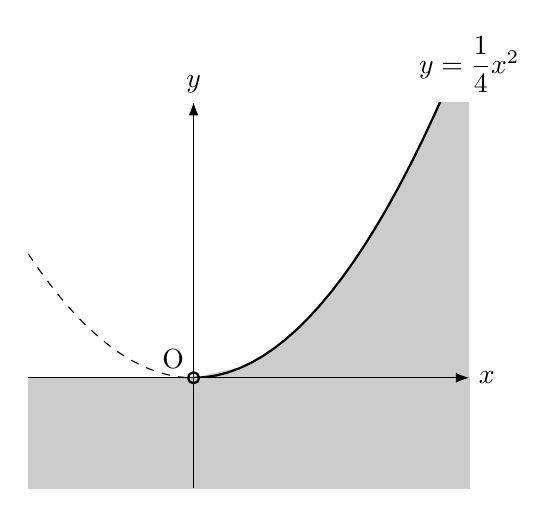
\begin{tikzpicture}[scale=0.7]
   
    \begin{scope}
        \clip(-3,0) rectangle (5,5);
        % Shade the region to the RIGHT of y = (1/4)x^2 within the clipped window
        \fill[black!20!white]
            (0,0)
            -- plot[domain=0:5] ({2*sqrt(\x)},{\x})
            -- (5,5)
            -- (5,0)
            -- cycle;
        \draw[thick] plot[domain=0:5] (\x,{1/4*pow(\x,2)}) node[below left]{$y=\dfrac{1}{4}x^2$};
    \end{scope}
        \filldraw[black!20!white](0,0)--(-3,0)--(-3,-2)--(5,-2)--(5,0)--cycle;
        \draw[dashed,domain=-3:0]plot(\x,{1/4*pow(\x,2)});
         \draw[->,>=Latex](-3,0)--(5,0)node[right]{$x$};
    \draw[->,>=Latex](0,-2)--(0,5)node[above]{$y$};
    \draw [thick] (0,0)circle[radius=0.1];
    \node[above left]at(0,0){O};
    \node[above]at(5,5){$y=\dfrac{1}{4}x^2$};
\end{tikzpicture}
\end{center}
求める領域は左図の網目部で原点を除き,$y=\dfrac{1}{4}x^2$上の境界以外すべて除く.\\\\
\kakkonib $\mathrm{P}(x,y)は方程式x^2+y^2\leq1 を満たす.またこのとき,\begin{cases}
    X=x+y\\
    Y=xy
\end{cases}とおくと,$
\begin{align*}
    (X,Y)\in W_2&\doti\exists(x,y),\begin{cases}
        X=x+y\\
        Y=xy\\
        x^2+y^2\leq1
    \end{cases}
    \doti\exists (x,y), \begin{cases}
        X=x+y\\
        Y=xy\\
        (x+y)^2-2xy\leq1
    \end{cases}\\
    &\doti \begin{cases}
        X^2-2Y\geq1\\
        \exists t,t^2-Xt+Y=0
    \end{cases}\doti \begin{cases}
        Y\geq \dfrac{X^2}{2}-\dfrac{1}{2}\\
        X^2-4Y\geq0
    \end{cases}\\
    &\doti\begin{cases}
        Y\geq\dfrac{X^2}{2}-\dfrac{1}{2}\\
        Y\leq\dfrac{X^2}{4}
    \end{cases} 
\end{align*}
これらを図示すると,下図の網目部が$W_2である.また,境界はすべて含む.$
\begin{center}
    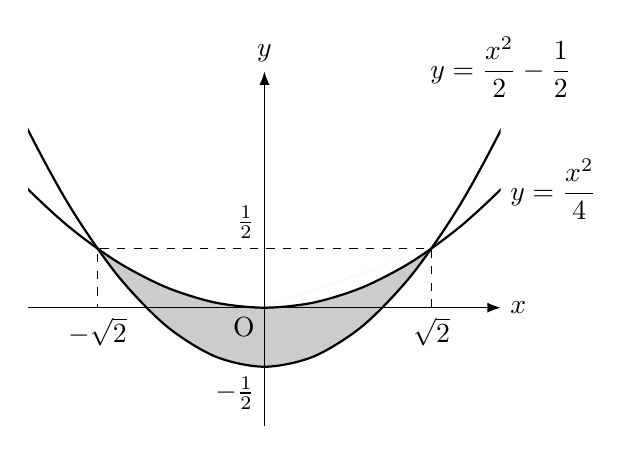
\begin{tikzpicture}[scale=1.5]
        
        \fill[black!20!white]
            (1.414,0.5)
            -- plot[domain=-1.414:1.414] (\x,{1/2*pow(\x,2)-1/2})
            -- (1.414,0.5)
            -- (0,0)
            -- plot[domain=1.414:-1.414] (\x,{1/4*pow(\x,2)});
            -- cycle;
        \draw[->,>=Latex](-2,0)--(2,0)node[right]{$x$};
        \draw[->,>=Latex](0,-1)--(0,2)node[above]{$y$};
        \begin{scope}
            \clip (-2,-1) rectangle (2,2);

        \draw[thick,smooth] plot(\x,{1/2*pow(\x,2)-1/2});
        \draw[thick,smooth] plot(\x,{1/4*pow(\x,2)});
        \end{scope}
        \node[above]at(2,1.7){$y=\dfrac{x^2}{2}-\dfrac{1}{2}$};
        \node[right]at(2,1){$y=\dfrac{x^2}{4}$};
        \draw[dashed](1.414,0)--(1.414,0.5)--(0,0.5)--(-1.414,0.5)--(-1.414,0)node[below]{$-\sqrt{2}$};
        \node[below]at(1.414,0){$\sqrt{2}$};
        \node[above left]at(0,0.5){$\frac{1}{2}$};
        \node[below left]at(0,-0.5){$-\frac{1}{2}$};
        \node[below left]at(0,0){O};
    \end{tikzpicture}
\end{center}
\newpage
\noindent\kakkosanb \begin{align*}
    (x,y)\in W_3&\doti\exists m,\begin{cases}
        (m-1)x-y+1=0\cdots\cdots\cdots\maruichi\\
        mx+(m-2)y+2=0\cdots\cdots\maruni\\
        m>0\cdots\cdots\cdots\cdots\cdots\cdots\cdots\cdots\cdots\cdots\marusan
    \end{cases}
\end{align*}
ここで$\maruichi より,$
\begin{align*}
    mx-x-y+1=0\doti m=\dfrac{x+y-1}{x} (x\neq0)
\end{align*}
なので,
\begin{align*}
    \exists m,\begin{cases}
        \maruichi\\
        \maruni\\
        \marusan
    \end{cases}&\doti \exists m,\begin{cases}
        m=\dfrac{x+y-1}{x} (x\neq0)\\
        m(x+y)-2y-2=0\\
        m>0
    \end{cases}\\\\
    &\doti \begin{cases}
        \dfrac{x+y-1}{x}(x+y)-2y-2=0\\
        \dfrac{x+y-1}{x}>0\\
        x\neq0
    \end{cases}\\\\
    &\doti \begin{cases}
        \dfrac{x^2+y^2+x-y}{x}=0\\
        x(x+y-1)>0\\
        x\neq0
    \end{cases}\\\\
    &\doti\begin{cases}
        \p{x+\dfrac{1}{2}}^2+\p{y-\dfrac{1}{2}}^2=\dfrac{1}{2}\\
        x(x+y-1)>0\\
        x\neq0
    \end{cases}
\end{align*}
これを図示すると,$\p{-\dfrac{1}{2},\dfrac{1}{2}}中心の円において,x\neq0より,y軸上の点を全て含まないことに注意して,次図を得る.$
\begin{center}
    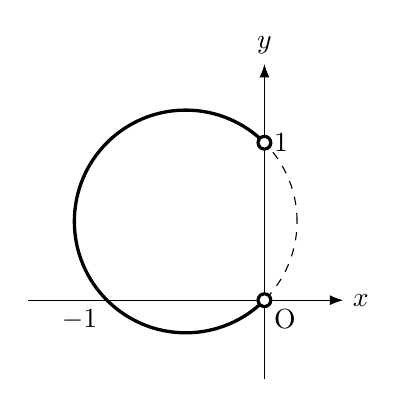
\begin{tikzpicture}[scale=2]
        \draw[->,>=Latex](-1.5,0)--(0.5,0)node[right]{$x$};
        \draw[->,>=Latex](0,-0.5)--(0,1.5)node[above]{$y$};
        \draw[dashed](-1/2,1/2)circle[radius=1/sqrt(2)];
        \node[below right]at(0,0){O};
        \draw
       [very thick] (0,1)circle[radius=0.04]; 
       \draw[very thick](0,0)circle[radius=0.04];
        \begin{scope}
            \clip (-1.5,-0.5) rectangle(0,1.25);
            \draw[very thick](-1/2,1/2)circle[radius=1/sqrt(2)];
            \node[below left]at(-1,0){$-1$};
        \end{scope}
        \node[right]at(0,1){1};
        \filldraw[thin,fill=white,draw=black](0,1)circle(1pt);
        \filldraw[fill=white,draw=black](0,0)circle(1pt);
    \end{tikzpicture}
\end{center}
$W_3は,左下図の太実線部で,原点,(1,0)を除き,それ以外の境界すべて含む.$\\\\
\kakkoshib \begin{align*}
    (x,y)\in W_4&\doti
        -1\leq\exists t\leq1,\begin{cases}
            x=2t-1\\
            y=t^2+t
        \end{cases}\\\\
        &\doti-1\leq \exists t\leq1,\begin{cases}
            t=\dfrac{x}{2}+\dfrac{1}{2}\\
            y=\dfrac{1}{4}x^2+x+1
        \end{cases}\\\\
        &\doti-1\leq\exists y\leq1\begin{cases}
            t=\dfrac{1}{2}(x+1)\\
            y=\dfrac{1}{4}x^2+x+1
        \end{cases}\\\\
        &\doti \begin{cases}
            -2\leq x+1\leq2\\
            y=\dfrac{1}{4}\p{x+2}^2
        \end{cases}\\\\
        &\doti\begin{cases}
            -3\leq x\leq1\\
            y=\dfrac{1}{4}\p{x+2}^2
        \end{cases}
\end{align*}
よって,下図を得る.
\begin{center}
    \begin{tikzpicture}
        \draw[->,>=Latex](-4,0)--(4,0)node[right]{$x$};
        \draw[->,>=Latex](0,-1)--(0,3.5)node[above]{$y$};
        \begin{scope}
            \clip (-4,0)rectangle(4,3.5);
            \draw[dashed]plot(\x,{1/4*pow(\x,2)+\x+1});
            \draw[very thick,domain=-3:1]plot(\x,{1/4*pow(\x,2)+\x+1});
            \draw[dashed](1,0)--(1,9/4)--(0,9/4)node[left]{$\frac{9}{4}$};
        \end{scope}
        \draw[dashed](-3,1/4)--(-3,0)node[below]{$-3$};
         \draw[dashed](1,9/4)--(1,0)node[below]{$1$};
         \node[below]at(-2,0){$-2$};
         \node[above left]at(0,1){$1$};
         \node[below left]at(0,0){O};
         \filldraw(-3,1/4)circle(2pt);
         \filldraw(1,9/4)circle(2pt);
    \end{tikzpicture}
\end{center}
$W_4は,上図の太実線部で,境界すべて含み,黒丸もすべて含む.$
\newpage
\noindent\ba{2.1.1}\\
\kai\\
\kakkoichib 2点P,Qを通る直線は,
\begin{align*}
    y&=\dfrac{8t}{8}(x-4)+2t^2+4t-1\\
    &=t(x-4)+2t^2+4t-1
\end{align*}
$\Y \kotaee{y=tx+3t^2-1}$\\\\
\kakkonib $領域Dを先に図示してから,2点\mathrm{A,B}がDに含まれないことを言う.$\\
$Dの表す式は,$
\begin{align*}
    \exists(x,y)\in D&\doti-1\leq\exists t\leq1,y=tx+2t^2-1\\
    &\doti -1\leq\exists t\leq1,2t^2+xt-y-1=0\\
    &\doti 二次関数f(t)=2t^2+xt-y-1が-1\leq t\leq1の範囲に少なくとも一つ実数解をもつ.
\end{align*}
$y=f(t)が,-1\leq t\leq1 に少なくとも一つ実数解を持つ条件をもつための条件は,下図を参照することにより,$
\begin{center}
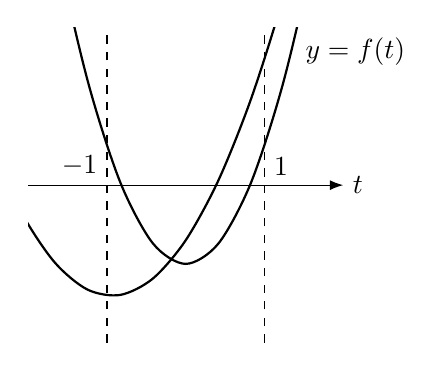
\begin{tikzpicture}
    \draw[->,>=Latex](-2,0)--(2,0)node[right]{$t$};
    \node[below right]at(1.4,2){$y=f(t)$};
    \begin{scope}
        \clip (-2,-2) rectangle(2,2);
        \draw[thick,smooth]plot(\x,{1.5*pow(\x,2)-1});
        \draw[dashed](-1,-2)--(-1,2);
        \draw[dashed](1,-2)--(1,2);
        \node[above left]at(-1,0){$-1$};
        \node[above right]at(1,0){1};
        \draw[thick,smooth]plot (\x,{0.8*pow(\x,2)+1.5*\x-0.7});
    \end{scope}
\end{tikzpicture}    
\end{center}
\begin{align*}
    f(-1)f(1)&\leq0(端点の積が異符号)または\begin{cases}
        (f(t)=0の判別式)x^2+8(y+1)\geq0\\
        -1<\frac{x}{4}<1\\
        f(-1)>0\\
        f(1)>0
    \end{cases}\\
    &\doti (-x-y+1)(x-y+1)\leq0 または\begin{cases}
        y<-x+1\\
        y<x+1\\
        -4<x<4\\
        y\geq-\frac{1}{8}x^2-1
    \end{cases}
\end{align*}
ところで,$y^\prime =-\dfrac{1}{2}xより,y=-\dfrac{1}{8}x^2-1は,
x=\pm4 でy^\prime=\mp1(復号同順)なので,x+y=1とx-y=-1とそれぞれx=\pm4で接する.これに注意して図示すると,次図がDである.$
\newpage
\begin{center}
    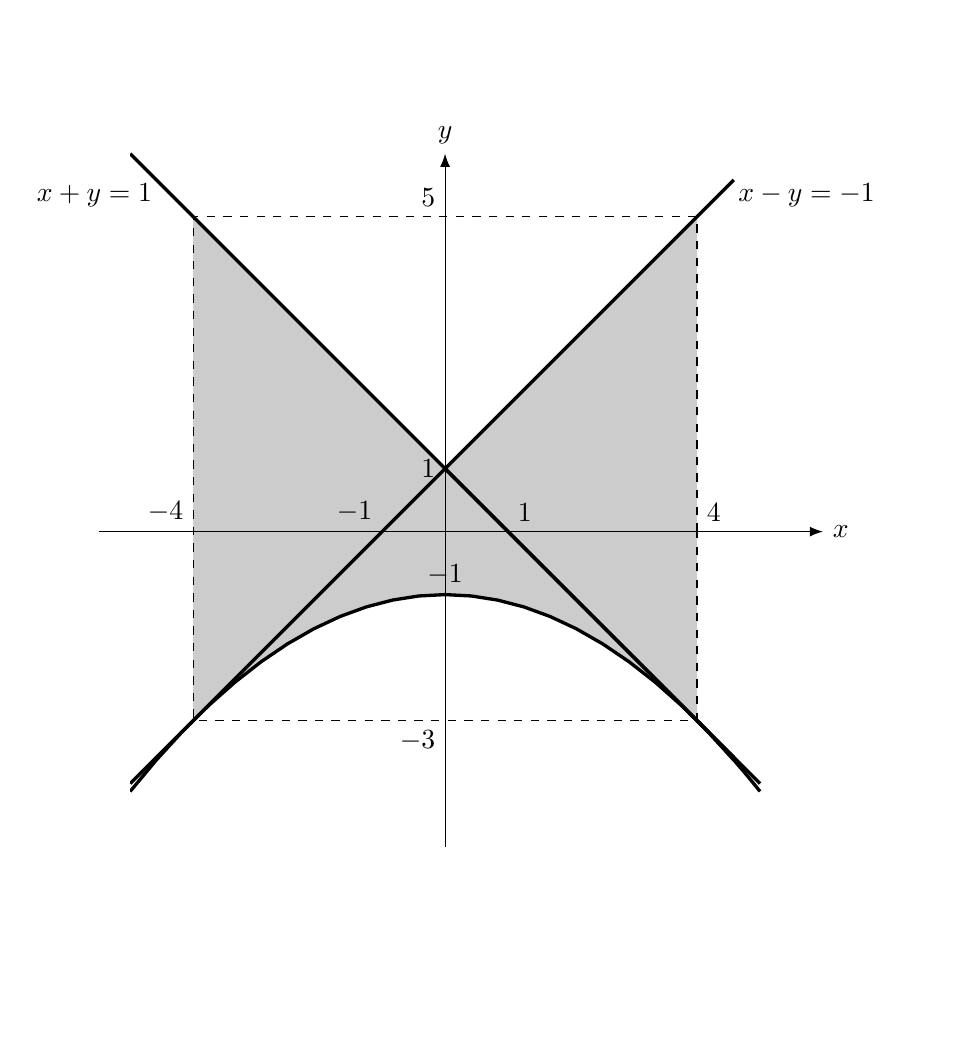
\begin{tikzpicture}[scale=0.8]
        \begin{scope}
            \clip(-5,-8)rectangle(8,8);
            \fill[black!20!white]
            (-4,5)
            --
            (-4,-3)
            --
            plot[domain=-4:4](\x,{-1/8*pow(\x,2)-1})
            --
            (4,5)
            --
            (0,1)
            --
            (-4,5)
            --cycle;
            \draw[very thick]plot(\x,{\x+1});
            \draw[very thick]plot(\x,{-\x+1});
            \draw[very thick]plot(\x,{-1/8*pow(\x,2)-1});
            \draw[dashed](4,0)--(4,5)--(-4,5)--(-4,-3)--(4,-3)--(4,0)node[above right]{4};
            \node[above left]at(-4,0){$-4$};
            \node[below left]at(0,-3){$-3$};
            \node[above right]at(1,0){$1$};
            \node[above]at(0,-1){$-1$};
            \node[above left]at(-1,0){$-1$};
            \node[ left]at(0,1){1};

        \end{scope}
        \draw[very thick,domain=4:5]plot(\x,{-1/8*pow(\x,2)-1});
         \draw[->,>=Latex](-5.5,0)--(6,0)node[right]{$x$};
        \draw[->,>=Latex](0,-5)--(0,6)node[above]{$y$};
        \draw[very thick,domain=0:5]plot(\x,{-\x+1});
         \node[above right]at(4.5,5){$x-y=-1$};
         \node[above left]at(-4.5,5){$x+y=1$};
         \node[above left]at(0,5){5};
    \end{tikzpicture}
\end{center}
上図の網目部が$Dで,\mathrm{A,B}は含まれない.$   \ans{(証明終わり)}\tokeiichi\\\\
$Dはy軸に関して対称なので,求める面積をSとおくと,$
\begin{align*}
    \dfrac{S}{2}&=-\dint{0}{4}\p{-\frac{1}{8}x^2-1}dx+(1+5)\cdot4\cdot\frac{1}{2}\\
    &=\frac{1}{24}\tint{x^3}{0}{4}+4+12\\
    &=\frac{8}{3}+16\\
    &=\frac{56}{3}
\end{align*}
$\Y S=\kotaee{\dfrac{112}{3}}$
\newpage
\noindent\fbox{\kurosankakub 類題演習2.1.2\kurosankakua}\\
\kai\\
\kakkoichib \begin{align*}
    2x^2+xy-y^2-4x+5y-6&=2x^2+x(y-4)-y^2+5y-6\\
    &=2x^2+x(y-4)-(y-2)(y-3)\\
    &=\B{x+\p{y-3}}\B{2x-\p{y-2}}\\
    &=\kotaee{(x+y-3)(2x-y+2)}
\end{align*}\\
\kakkonib $D:(2x+y-3)(x-y+2)>0を描く.$\\
$(x,y)=(0,0)\nein Dなので,Dの表す領域は下図の網目部となり,境界はすべて除く.$
\begin{center}
    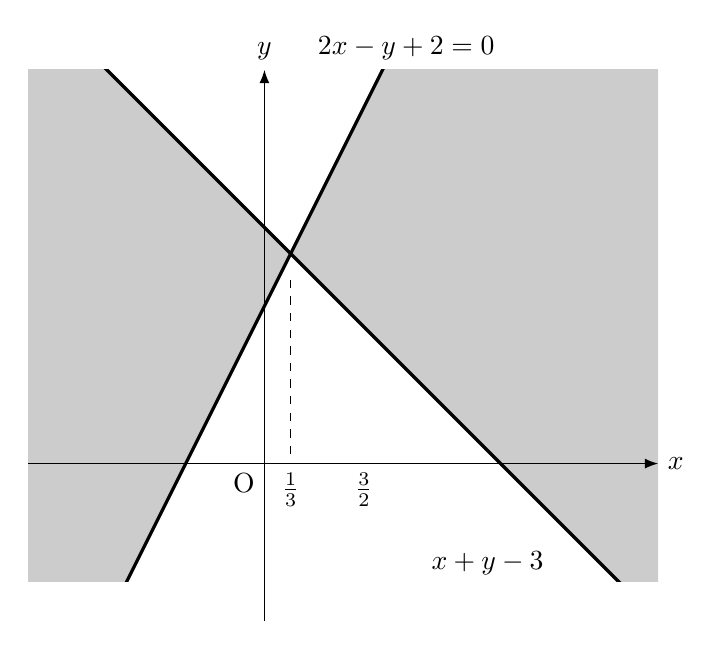
\begin{tikzpicture}
    \begin{scope}
        \clip (-3,-1.5)rectangle(5,5);
        
        \node[below right]at(-2,0){$-2$};
        \node[below left]at(3/2,0){$\frac{3}{2}$};
        \node[below left]at(0,0){O};
        \fill[black!20!white]
        (1/3,8/3)
        --
        plot[domain=1/3:5](\x,{-\x+3})
        --
        plot[domain=5:1/3](\x,{2*\x+2})
        --
        (1/3,8/3)
        --cycle;
        \fill[black!20!white]
        (1/3,8/3)
        --
        plot[domain=1/3:-3](\x,{-\x+3})
        --
        plot[domain=-3:1/3](\x,{2*\x+2})
        --
        (1/3,8/3)
        --cycle;
        \draw[very thick]plot(\x,{-\x+3});
        \draw[very thick]plot(\x,{2*\x+2});
    \end{scope}
    \draw[->,>=Latex](-3,0)--(5,0)node[right]{$x$};
    \draw[->,>=Latex](0,-2)--(0,5)node[above]{$y$};
    \node[above]at(1.8,5){$2x-y+2=0$};
    \node[below right]at(2,-1){$x+y-3$};
    \draw[dashed](1/3,7/3)--(1/3,0)node[below]{$\frac{1}{3}$};
     \end{tikzpicture}
    \end{center}
    \kakkoshib \begin{align*}
    x^2+y^2-2kx-y+k^2<0 &\doti \p{x-k}^2+\p{y-\dfrac{1}{2}}^2<\dfrac{1}{4}\\
    &\doti 中心\p{k,\dfrac{1}{2}},半径\dfrac{1}{2}の円の内部.
\end{align*}
これより,$D\cap E=\emptyset となるkの下限値と上限値はそれぞれ,$
\begin{center}
    $x-y=-2とEが接するとき.(下限値)$\\
    $2x+y=3とEが接するとき.(上限値)$
\end{center}
である.これより,$Eと\kakkoichib を同一平面内で図示して,下限値と上限値の状態を描くと,図は次のような図になる.$
\newpage
\begin{center}
    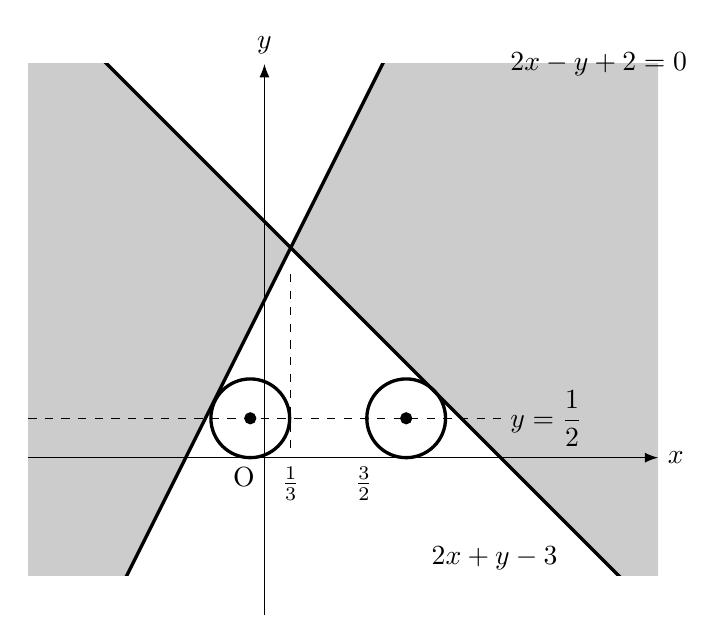
\begin{tikzpicture}
    \begin{scope}
       \clip (-3,-1.5)rectangle(5,5);
        
        \node[below right]at(-2,0){$-2$};
        \node[below left]at(3/2,0){$\frac{3}{2}$};
        \node[below left]at(0,0){O};
        \fill[black!20!white]
        (1/3,8/3)
        --
        plot[domain=1/3:5](\x,{-\x+3})
        --
        plot[domain=5:1/3](\x,{2*\x+2})
        --
        (1/3,8/3)
        --cycle;
        \fill[black!20!white]
        (1/3,8/3)
        --
        plot[domain=1/3:-3](\x,{-\x+3})
        --
        plot[domain=-3:1/3](\x,{2*\x+2})
        --
        (1/3,8/3)
        --cycle;
        \draw[very thick]plot(\x,{-\x+3});
        \draw[very thick]plot(\x,{2*\x+2});
        
        
    \end{scope}
    \draw[->,>=Latex](-3,0)--(5,0)node[right]{$x$};
    \draw[->,>=Latex](0,-2)--(0,5)node[above]{$y$};
    \node[right]at(3,5){$2x-y+2=0$};
    \node[below right]at(2,-1){$2x+y-3$};
    \draw[dashed](1/3,7/3)--(1/3,0)node[below]{$\frac{1}{3}$};
    \draw[very thick](-0.18,1/2)circle[radius=1/2];
    \filldraw(-0.18,1/2)circle(2pt);
    \draw[very thick] (1.8,1/2)circle[radius=1/2];
    \filldraw(1.8,1/2)circle(2pt);
 \draw[dashed](-3,1/2)--(3,1/2)node[right]{$y=\dfrac{1}{2}$};
     \end{tikzpicture}
    \end{center}
点と直線の距離公式より,Eとそれぞれの直線が接するなら,中心からの距離と半径が一致するので,まず下限値は,
\begin{align*}
    \dfrac{\left|2k-\frac{1}{2}+2\right|}{\sqrt{2^2+1}}=\dfrac{1}{2}&\doti \left|2k+\dfrac{3}{2}\right|=\dfrac{\sqrt{5}}{2}\\
    &\doti k=\dfrac{-3\pm\sqrt{5}}{4}\cdots\cdots\cdots\cdots\maruichi 
\end{align*}
である.また上限値は,
\begin{align*}
    \dfrac{\left| k+\frac{1}{2}+3\right|}{\sqrt{1+1}}=\dfrac{\sqrt{2}}{2}&\doti \left|k-\dfrac{5}{2}\right|=\dfrac{\sqrt{2}}{2}\\
    &\doti k=\dfrac{5\pm\sqrt{2}}{2}\cdots\cdots\cdots\cdots\maruni  
\end{align*}
$\maruichi,\maruni  より,D\cap E=\emptyset になるためには下限値が,k>-1,上限値が,k<\dfrac{3}{2}をそれぞれ満たす必要があるので,
求めるkの値の範囲は,$
\begin{align*}
    \kotaee{\dfrac{-3+\sqrt{5}}{4}\leq k\leq\dfrac{5-\sqrt{2}}{2}}
\end{align*}
\newpage
\noindent\ba{2.2.0}\\
\kangaekata\\
\kakkoichi  は情報不足により,解答することができなくなっています.\\
\kakkoni 内積の不等式を使えそうな形ですが,大きさの計算の部分で$x+7y=1を出すことができません.視点を変えて,\ans{1}に注目してみると
\dfrac{1}{7x}+\dfrac{1}{y}にx+7yを掛け算しても良いことになります.$\\
\kakkosan 分子の次数は分母の次数より大きいので,字数下げをしないと始まりません.\\
\kakkoshi  全力展開!!\\
\kai\\
\kakkoichib 解答不能.\\\\
\kakkonib $\dfrac{1}{7x}+\dfrac{1}{y}にx+7yをかけると,$
\begin{align*}
    (x+7y)\p{\dfrac{1}{7x}+\dfrac{1}{y}}&=\dfrac{1}{7}+\dfrac{x}{y}+\dfrac{y}{x}+7\\
    &\geq 7+\dfrac{1}{7}+2\sqrt{\dfrac{x}{y}\cdot\dfrac{y}{x}}\\
    &=9+\dfrac{1}{7}=\dfrac{64}{7}
\end{align*}
等号は,$\dfrac{x}{y}=\dfrac{y}{x}\doti x=y=\dfrac{1}{8}\p{\because x+7y=1\doti 8y=8x=1}のとき成立する.$\\
$\Y 求める最小値は,\kotaee{\dfrac{64}{7}}$\\\\
\kakkosanb $\spadesuit 分子の次数が分母の次数より大きいので,次数下げをしましょう.そこから,項が三つの\mathrm{AM-GM}の関係を使います.\spadesuit$\\
$f(x)=\dfrac{x^3+3x^2+3x+5}{x^2+2x+1}とおくと,$
\begin{align*}
    f(x)&=\dfrac{(x+1)^3+4}{(x+1)^2}\\
    &=x+1+\dfrac{4}{(x+1)^2}\\
    &=\dfrac{x+1}{2}+\dfrac{x+1}{2}+\dfrac{4}{(x+1)^2}\geq3\cdot\sqrt[3]{\dfrac{x+1}{2}+\dfrac{x+1}{2}+\dfrac{4}{(x+1)^2}}=3 (\because\mathrm{AM-GM})
\end{align*}
また等号は,
\begin{align*}
    \dfrac{x+1}{2}=\dfrac{4}{x+1}\doti x+1=2 のとき成立.
\end{align*}
$\Y\kotaee{\min f(x)=3}$\\\\
\newpage
\noindent\kakkoshib 
\begin{align*}
    \p{\dfrac{1}{x}+\dfrac{1}{y}+\dfrac{1}{z}}\p{x+y+z}&=3+\dfrac{x}{y}+\dfrac{y}{x}+\dfrac{x}{z}+\dfrac{z}{x}+\dfrac{y}{z}+\dfrac{z}{y}\\
    &\geq 3+2\sqrt{\dfrac{x}{y}\cdot\dfrac{y}{x}}+2\sqrt{\dfrac{x}{z}\cdot\dfrac{z}{x}}+2\sqrt{\dfrac{y}{z}\cdot\dfrac{z}{y}}=9 (\because \mathrm{AM-GM})
\end{align*}
$また等号は,$
\begin{align*}
    \dfrac{x}{y}=\dfrac{x}{x}かつ\dfrac{x}{z}=\dfrac{z}{x}かつ\dfrac{y}{z}=\dfrac{z}{y}\doti x=y=z のとき成立する.
\end{align*}
$\Y 最小値は,\kotaee{9}$\\\\
\fbox{\kurosankakub 類題演習2.2.1\kurosankakua}\\
\kai\\
\kakkoichib $\p{x+\dfrac{1}{y}}\p{y+\dfrac{4}{x}}=xy+\dfrac{4}{xy}+5\geq 4+5 (\because \mathrm{AM-GM})\\
等号は,xy=\dfrac{4}{xy}\doti xy=2のとき成立する.$\\
$\Y 最小値は,\kotaee{9}$\\\\
\kakkonib $f(x)=\dfrac{x+2}{x^2+2x+16}\cdots\cdots\cdots\maruichi とおく.x\neq0なので,\maruichi の両辺に逆数をとると,$
\begin{align*}
    \dfrac{1}{f(x)}&=\dfrac{x^2+2x+16}{x+2}=x+\dfrac{16}{x+2}\\
    &=(x+2)+\dfrac{16}{x+2}-2\geq8-2=6(\because\mathrm{AM-GM})
\end{align*}
また,等号成立は,\begin{align*}
    x+2=\dfrac{16}{x+2}\doti x=2のとき成立する.
\end{align*}
$\Y \dfrac{1}{f(x)}の最小値は6なので,f(x)の最小値は\kotaee{\dfrac{1}{6}}$\\\\
\kakkosanb $\mathrm{AM-GM}の関係より,$
\begin{align*}
    x+\dfrac{2}{x}\geq2\sqrt{2} (等号成立は,x=\sqrt{2})
\end{align*}
これより,
\begin{align*}
    \p{x+\dfrac{2}{x}}^6\geq512
\end{align*}
なので,常に$\p{x+\dfrac{2}{x}}^6\geq yが成り立つための条件は,y\leq512$\\
$\Y 最大値は,\kotaee{512}$
\newpage
\subsection{第3回}
\noindent\ba{3.1.0}\\
\kangaekata\\
\kakkoshi は積分だけで面積を求めることができないので,\ans{大きい面積から余分な面積を引く.}ことを考えましょう!!また,面積の計算結果は汚くなることが多いです.数学\suII だと面積計算は出題されにくいので,一応注意しておきます.\\
\kai\\
\kakkoichib,\kakkonib $\mathrm{A}\p{\sqrt{3},-\dfrac{1}{2}}をKの式に代入すると,$
\begin{align*}
    \dfrac{3}{4}+\dfrac{1}{4}=r^2\doti \kotaee{r=1}
\end{align*}
また,$\mathrm{A}での接線の方程式は,$
\begin{align*}
    y=\sqrt{3}\p{x-\sqrt{3}}-\dfrac{1}{2}\doti\kotaee{y=\sqrt{3}x-\dfrac{7}{2}}
\end{align*}
ところで,Cについて$y^\prime=2ax より,\mathrm{A}での接線の傾きは一致するので$
\begin{align*}
    2\sqrt{3}a=\sqrt{3}\doti\kotaee{a=\dfrac{1}{2}}
\end{align*}
このとき,
\begin{align*}
    -\dfrac{1}{2}=3a+b\doti\kotaee{b=-2}
\end{align*}\\
\kakkosanb
\begin{align*}
    \dint{-2}{\sqrt{3}}(ax^2+b)dx&=\tint{\dfrac{a}{3}x^3+bx}{-2}{\sqrt{3}}\\
    &=\dfrac{a}{3}\p{3\sqrt{3}+8}+b\p{\sqrt{3}+2}\\
    &=\dfrac{1}{6}\p{3\sqrt{3}+8}-2\sqrt{\sqrt{3}+2}\\
    &=\kotaee{-\dfrac{3\sqrt{3}}{2}-\dfrac{8}{3}}
\end{align*}\\
\kakkoshib 表す領域を$D$とする.すなわち,
\begin{align*}
    D:\begin{cases}
        x\leq\sqrt{3},y\leq0,y\geq\frac{1}{2}x^2-2\\
        \p{x-\dfrac{\sqrt{3}}{2}}^2+y^2\geq1
    \end{cases}
\end{align*}
これを図示すると次図のようになる.
\newpage
\begin{center}
    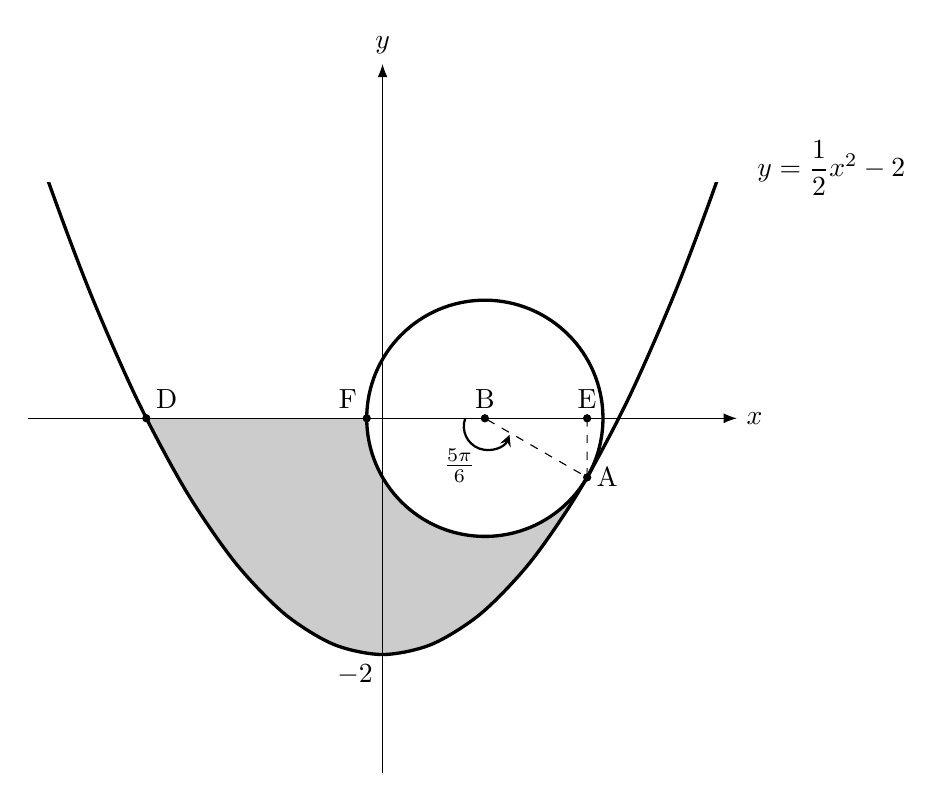
\begin{tikzpicture}[scale=1.5]
        
        \coordinate(D)at(-2,0);
        \coordinate(E)at({sqrt(3)},{-1/2});
        \coordinate(B)at({sqrt(3)/2},0);
        \coordinate(F)at({-1+sqrt(3)/2},0);
        \coordinate(A)at({sqrt(3)},{-1/2});
        \begin{scope}
            \clip (-3,-2.2)rectangle(3,2);
        \fill[black!20!white,even odd rule]
        (D)
        -- plot[smooth,domain=-2:{sqrt(3)},samples=300] (\x,{1/2*\x*\x-2})
        -- (E)
          arc[start angle=-30,end angle=180,radius=1]
        -- (F) -- cycle
        ({sqrt(3)/2},0) circle[radius=1];
        \draw[smooth,very thick]plot(\x,{1/2*pow(\x,2)-2});
        \draw[very thick] ({sqrt(3)/2},0)circle[radius=1];
                \end{scope}
\draw[->,>=Latex](-3,0)--(3,0)node[right]{$x$};
        \draw[->,>=Latex](0,-3)--(0,3)node[above]{$y$};
        \node[above]at(B){B};
        \fill(B)circle(1pt);
        \node[right]at(E){A};
        \fill(E)circle(1pt);
        \node[above]at({sqrt(3)},0){E};
        \fill({sqrt(3)},0)circle(1pt);
        \node[above left]at(F){F};
        \fill(F)circle(1pt);
        \node[above right]at(D){D};
        \fill(D)circle(1pt);
        \node[below left]at(0,-2){$-2$};
        \node[above]at(3.8,1.8){$y=\dfrac{1}{2}x^2-2$};
        \draw[dashed]({sqrt(3)},0)--(E)--(B);
        \draw [thick,->,>=stealth](0.7,0) arc [start angle = -200, end angle = -21, radius = 0.2];
        \node[left]at({sqrt(3)/2},-0.4){$\frac{5\pi}{6}$};
    \end{tikzpicture}  
\end{center}
上図のように点$\mathrm{A}\p{\sqrt{3},-\dfrac{1}{2}},\mathrm{B}\p{\dfrac{\sqrt{3}}{2},0},\mathrm{D}\p{-2,0},\mathrm{E}\p{\sqrt{3},0},
\mathrm{F}:Cとx軸の交点 とおく.$\\
また$\Sankaku{ABE}は\mathrm{AE}:\mathrm{EB}=\dfrac{1}{2}:\dfrac{\sqrt{3}}{2}=1:\sqrt{3}の直角三角形なので,\Kaku{DBA}=\pi-\dfrac{\pi}{6}=\dfrac{5\pi}{6}である.$\\
よって,$求める面積Sは,$
\begin{align*}
    S&=\dint{-2}{\sqrt{3}}\B{-\p{ax^2+b}}dx-扇形\mathrm{FBA}-\Sankaku{ABE}\\
    &=\dfrac{3\sqrt{3}}{2}+\dfrac{8}{3}-1^2\cdot\pi\cdot\dfrac{150\ddo}{360\ddo}-\dfrac{1}{2}\cdot\dfrac{\sqrt{3}}{2}\cdot\dfrac{1}{2}\\
    &=\dfrac{3\sqrt{3}}{2}+\dfrac{8}{3}-\dfrac{5\pi}{12}-\dfrac{\sqrt{3}}{8}\\
    &=\kotaee{\dfrac{11\sqrt{3}}{3}+\dfrac{8}{3}-\dfrac{5\pi}{12}}
\end{align*}
\newpage
\noindent\ba{3.1.1}\\
\kangaekata\\
\kakkoni はもともと$aの存在条件を同値変形する問題ですが,\mathrm{AB}の中点がaで表せないので,適当な文字で\mathrm{A,B}の座標を置くことから始めます.$\\
\kai\\
$\begin{cases}
    y=x^2\cdots\cdots\cdots\cdots\cdots\cdots\cdots\cdots\maruichi\\
    y=-x^2+2ax-a\cdots\cdots\maruni
\end{cases}$\\
\kakkoichib $2曲線の交点異なる二つの共有点の持つための条件は,\maruichi=\maruni より,2x^2-2ax+a=0\cdots\cdots\marusan の判別式が正であることなので$
\begin{align*}
  (\marusan の判別式)a^2-2a>0\doti\kotaee{a<0,a>2}
\end{align*}
\kakkonib $\mathrm{A,B}の中点のx座標をそれぞれ,X_1,X_2とおくと,\mathrm{AB}の中点の座標\mathrm{M}は\mathrm{M}\p{\dfrac{X_1+X_1}{2},\dfrac{(X_1+X_2)^2}{2}}とおける.$\\
$ここで,X_1,X_2は\maruichi の異なる2つの実数解なので,解と係数の関係より,$
\begin{align*}
    \begin{cases}
        X_1+X_2=1\\
        X_1X_2=\frac{a}{2}
    \end{cases}
\end{align*}
$\mathrm{M}\p{\dfrac{a}{2},\dfrac{a^2-a}{2}}であり,更にX=\dfrac{a}{2},Y=\dfrac{a^2-a}{2}とし,\mathrm{M}の軌跡をWとすると,$
\begin{align*}
    (X,Y)\in W&\doti\exists a,\begin{cases}
        X=\frac{a}{2}\\
        Y=\frac{a^2-a}{2}\\
        a<0,a>2
    \end{cases}\\
    &\doti\begin{cases}
        Y=X^2-X\\
        X<0,X>4
    \end{cases}\\
    &\doti Wはy=x^2-xのx<0,x>4の部分.
\end{align*}
これを図示すると下図の太実線部が$Wで,白丸を除く.$
\begin{center}
    \begin{tikzpicture}[scale=1.3]
        \draw[->,>=Latex](-2,0)--(4,0)node[right]{$x$};
        \draw[->,>=Latex](0,-1)--(0,5)node[above]{$y$};
        \begin{scope}
            \clip (-2,-1)rectangle(3,5);
            \draw[dashed,smooth]plot(\x,{pow(\x,2)-\x});
            \draw[very thick,smooth,domain=2:3]plot(\x,{pow(\x,2)-\x});
            \draw[very thick,smooth,domain=0:-2]plot(\x,{pow(\x,2)-\x});
            \filldraw[fill=white,draw=black](0,0)circle(2.5pt);
            \filldraw[fill=white,draw=black](2,2)circle(2.5pt);
            \node[below left]at(0,0){O};
            \draw[dashed](2,2)--(2,0)node[below]{$4$};
            

            
         \end{scope}
         \node[right]at(3,5.5){$y=x^2-x$};
    \end{tikzpicture}
\end{center}
\newpage
\noindent\fbox{類題演習3.1.2}\\
\kangaekata\\
頻出の交点の軌跡の問題です.軌跡なので,普通に存在条件に帰着させれば良いですが,場合分けを忘れないようにしましょう.\\
\kai
\begin{align*}
    \begin{cases}
        mx-y=1\cdots\cdots\cdots\maruichi\\
        x+my=m+2\cdots\cdots\cdots\maruni
    \end{cases}
\end{align*}
$\maruichi,\maruni の交点を(X,Y)とし,交点の軌跡Wとする.$
\begin{align*}
    (X,Y)\in W&\doti
     \exists m,\begin{cases}
        mX-Y=1\\
        X+mY=m+2
    \end{cases}\cdots\cdots\cdots\asta
\end{align*}
\tokeiichi\underline{$X=0のとき$}
\begin{align*}
    \asta&\doti \exists m,\begin{cases}
        -Y=1\\
        mY=m+2
    \end{cases}\doti m=-1
\end{align*}
\tokeini\underline{$X\neq0 のとき$}
\begin{align*}
    \asta&\doti \exists m,\begin{cases}
        m=\frac{y+1}{x}\\
        \maruni
    \end{cases}\doti\frac{x^2+y^2-2x-1}{x}=0\\
    &\doti x\B{(x-1)^2+y^2-2}=0
\end{align*}
よって,$Wは下図の太実線部で,白丸を除く.$
\begin{center}
    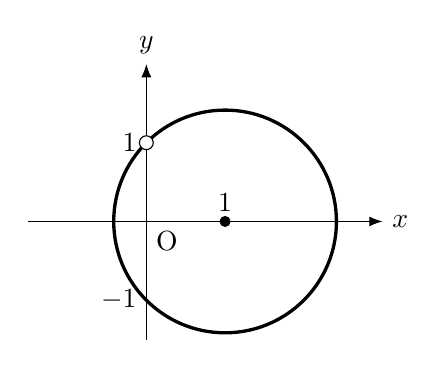
\begin{tikzpicture}
        \draw[->,>=Latex](-1.5,0)--(3,0)node[right]{$x$};
        \draw[->,>=Latex](0,-1.5)--(0,2)node[above]{$y$};
        \draw[very thick](1,0)circle[radius={sqrt(2)}];
        \filldraw[fill=white,draw=black](0,1)circle(2.5pt);
        \node[below right]at(0,0){O};
        \node[left]at(0,1){1};
        \node[left]at(0,-1){$-1$};
        \fill(1,0)circle(2pt);
        \node[above]at(1,0){1};
    \end{tikzpicture}
\end{center}
\newpage
\subsection{第4回}
\noindent\ba{4.1.0}\\
\kangaekata\\
\kakkoichi では,割り算の性質$P(x)\godo0\kmod{x^2-1}\doti P(x)\godo0\kmod{x-1}かつP(x)\godo0\kmod{x+1} を用います.$\\
\kakkosan 素因数分解をさせた意味を考えましょう.\\
\kai\\
\kakkoichib $x^2-1=(x-1)(x+1)なので,$
\begin{align*}
\begin{cases}
    P(x)\godo0\kmod{x-1}\\
    P(x)\godo0\kmod{x+1}
\end{cases}を示す.
\end{align*}
いま,$ x^2\godo x^5\godo x^4\godo x^3\godo\cdots\godo 1\kmod{x-1}$
なので,
\begin{align*}
    P(x)&\godo(1-3+3-1)\cdot1\cdot2\cdot3\cdot4\\
    &\godo 0\kmod{x-1}
\end{align*}
同様に,$x^6\godo-x^5\godo x^4\godo-x^3\godo\cdots\godo1\kmod{x+1}$より,$P(x)\godo0\kmod{x+1}$\\
$\Y \begin{cases}
    P(x)\godo0\kmod{x-1}\\
    P(x)\godo0\kmod{x+1}
\end{cases}\doti P(x)\godo0\kmod{x^2-1} \ans{(証明終わり)}$\\\\
\kakkonib
\begin{align*}
6480&=10\times648=10\times4\times162=10\times4\times2\times81\\
&=2^4\times5\times9^2\\
&=\kotaee{2^4\times3^4\times5}
\end{align*}\\
\kakkosanb $P(n)=(n^6-3n^4+3n^2-1)n^3(n^2+1)(n^2+2)(n^2+3) と因数分解できるので,$
\begin{align*}
    \begin{cases}
        P(n)\godo0\kmod{2^4}\cdots\cdots\cdots\maruichi\\
        P(n)\godo0\kmod{3^4}\cdots\cdots\cdots\maruni\\
        P(n)\godo0\kmod{5}\cdots\cdots\cdots\marusan
    \end{cases}
\end{align*}
であることをそれぞれ言えばよい.\\
\newpage
まず,$\maruichi$ を示す.合同式の対称性に注目して下表を得る.
\begin{center}
    \begin{tabular}{|c||c|c|c|c|c|c|c|c|}
        \hline
        $n\kmod{16}$ & $0$ & $\pm1$ & $\pm2$ & $\pm3$ & $\pm4$ & $\pm5$ & $\pm6$ & $\pm7$\\
        \hline
        $n^2\kmod{16}$ & $0$ & $1$ & $4$ & $9$ & $0$ & $9$ & $4$ & $1$ \\
        \hline
        $n^4\kmod{16}$ & $0$ & $1$ & $0$ & $1$ & $0$  & $1$ & $0$ & $1$ \\
        \hline
        $n^6\kmod{16}$ & $0$ & $1$ & $0$ & $1$ & $0$  & $1$ & $0$ & $1$ \\
        \hline
        $P(n)\kmod{16}$ & $0$ & $0$ & $0$ & $0$ & $0$  & $0$ & $0$ & $0$ \\
        \hline
    \end{tabular}
\end{center}
上表より,$\maruichi が示された.$\\
 $\maruni を示す.\\
n\geq 2なので,P(n)の最小値は$
\begin{align*}
    P(2)&=(64-48+12-1)\times2^3\times5\times6\times7=27\times3\times2^4\times5\times7\\
    &=81\times2^4\times5\times7>81
\end{align*}
なので,$P(n)\godo0\kmod{9}を言えば十分である.これより,下表を得る.$
\begin{center}
    \begin{tabular}{|c||c|c|c|c|c|}
        \hline
        $n\kmod{9}$ & $0$ & $\pm1$ & $\pm2$ & $\pm3$ & $\pm4$\\
        \hline
        $n^2\kmod{9}$ & $0$ & $1$ & $4$ & $0$ & $7$\\
        \hline
        $n^4\kmod{9}$ & $0$ &  $1$ & $7$ & $0$ & $49\godo4$\\
        \hline
        $n^6\kmod{9}$ & $0$ & $1$ & $28\godo1$ & $0$ & $28\godo1$\\
        \hline
        $P(n)\kmod{9}$ & $0$& $0$& $0$& $0$& $0$\\
        \hline
        
    \end{tabular}
\end{center}
上表より,$\maruni が示された.$\\
 最後に$\marusan を示す.$
\begin{center}
    \begin{tabular}{|c||c|c|c|}
        \hline
        $n\kmod{5}$ & $0$ & $\pm1$ & $\pm2$ \\
        \hline
        $n^2\kmod{5}$ & $0$ & 1 & 1\\
        \hline
        $n^4\kmod{5}$ & $0$ & $1$ & $16\godo1$\\
        \hline
        $n^6\kmod{5}$ & $0$ & $1$ & $4$\\
        \hline
        $P(n)\kmod{5}$ & $0$ & 0 &$n^2+1\godo0$\\
        \hline
    \end{tabular}
\end{center}
上表より,$\marusan が示された.$\\
$\Y 以上\maruichi 〜\marusan よりP(n)\godo0\kmod{6480}である.\ans{(証明終わり)}$
\newpage
\noindent\ba{4.1.1}\\
\kangaekata\\
かなりの難問です.\kakkoichi では$\kmod{5}で考えて周期性を見つけて終わりです.\kakkoni はb_nを5で割った余りは問題で与えられている文字
だけでは表せないので,新たにb_nを5で割った商と余りを文字で設定します.\kakkosan は\kakkoni ができればいけます.$\\
\kai\\
\kakkoichib 以下,合同式の法を5で考える.
\begin{align*}
&a_1=8=5\cdot1+3\godo3\\
&a_2=2a^2_1+1\godo2\cdot16+1\godo4\\
&a_3=2a_2^2+1\godo2\cdot16+1\godo3\\
&a_4=2a_3^3+1\godo2\cdot9+1\godo4\\
&\vdots
\end{align*}
よって,$r_nは\mod5で3と4を周期的に繰り返し,$
   $\kotaee{r_n= \begin{cases}
    3 (n:奇数)\\
    4 (n:偶数)
    \end{cases}}$\\\\
\kakkonib $a_n=5b_n+r_nをa_{n+1}=2a_n^2+1\cdots\cdots\cdots\maruichi に代入すると,$
\begin{align*}
a_{n+1}&=2(5b_n+r_n)^2+1=2(25b_n^2+10b_nr_n+r_n^2)+1\\
&=5(10b_n^2+4b_nr_n)+2r_n^2+1\cdots\cdots\cdots\maruni
\end{align*}
ここで,$b_nを5で割った商をc_n,余りをs_nとおくと,b_n=5c_n+s_nと表せる.このことと,\kakkoichi の結果より,$\\
\tokeiichi\underline{$nが奇数\doti r_n=3のとき$}\\
 $\maruni  より,a_{n+1}=5(10b_n^2+12b_n)+19\cdots\cdots\cdots\marusan なので,$
\begin{align*}
    b_{n+1}&=10b_n^2+12b_n+3=10b_n^2+12(5c_n+s_n)+3\\
    &\godo2s_n+3\kmod{5}
\end{align*}
よって,$s_{n+1}は2s_n+3を5で割った余りに等しい.$\\
\tokeini\underline{$nが偶数\doti r_n=4のとき$}\\
 $\maruni より,a_{n+1}=5(10b_n^2+16b_n)+33\cdots\cdots\cdots\marushi なので,$
\begin{align*}
    b_{n+1}&=10b_n^2+16b_n+6\\
    &=10b_n^2+16(5c_n+s_n)+6\\
    &\godo s_n+1\kmod{5} (続きは次ページ)
\end{align*}
よって,$s_{n+1}はs_n+1を5で割った余りに等しい.$\\
$\Y 以上をまとめると,$
\begin{align*}
    &r_n=3(\doti nが奇数)\narabaa b_{n+1}\godo2s_n+3\kmod{5}\\
    &r_n=4(\doti nが偶数)\narabaa b_{n+1}\godo s_n+1\kmod{5}
\end{align*}
また,$b_1=1より,s_1=1なので,$
\begin{align*}
    &\p{s_n,r_n}=(1,3)のとき,\p{s_{n+1},r_{n+1}}=(0,4)\\
    &\p{s_n,r_n}=(0,4)のとき,\p{s_{n+1},r_{n+1}}=(1,3)
\end{align*}
となって,$\p{s_n,r_n}は(0,4),(1,3)を周期的に繰り返す.$\\
$\Y \kotaee{s_n=\begin{cases}
    0 (n:偶数)\\
    1 (n:奇数)
\end{cases}}$
\kakkosanb $まず,\marusan よりnが奇数なので,$
\begin{align*}
    a_{n+1}&=50b_n^2+60b_n+19\\
    &=50b_n^2+60(5c_n+1)+19\\
    &\godo10+19\kmod{50}\\
    =29
\end{align*}
次に$\marushi より,nが偶数なので,$
\begin{align*}
    a_{n+1}&=50b_n^2+60b_n+33\\
    &=50b_n^2+60\cdot5c_n+33\\
    &\godo33\kmod{50}
\end{align*}
また,$a_1=8に注意して,a_nを50で割った余りは,
\kotaee{
    \begin{cases}
8 (n=1)\\
29 (n:偶数)\\
33 (n:3以上の奇数)
\end{cases}}$
\newpage
\noindent\fbox{\kurosankakub 類題演習4.1.2\kurosankakua}\\
\kangaekata\\
\Bc{ア}:整数や数列の問題で,よく分からない問題はとりあえず実験しましょう.\\
\Bc{イ}: この問題は「穴埋め」問題なので,しっかりとした記述は必要ありませんが,記述できるようにしておきましょう.\kakkoichi での実験から$n=5までの積が最大に
なることがわかります.ですが根拠がありません.すなわち,\ans{n\geq6でa_nが1より小さい単調減少な数列である.}ことを言う必要があります.$\\
\kai\\
\Bc{ア}: 
\begin{align*}
    &a_1=2\cdot3\cdot4=24\\
    &a_2=\dfrac{3\cdot4\cdot5}{2!}=30\\
    &a_3=\dfrac{4\cdot5\cdot6}{3!}=20\\
    &a_4=\dfrac{5\cdot6\cdot7}{4!}=\dfrac{35}{4}\\
    &a_5=\dfrac{6\cdot7\cdot8}{5!}=\dfrac{14}{5}\\
    &a_6=\dfrac{7\cdot8\cdot9}{6!}=\dfrac{7}{10}<1\\
    &\vdots
\end{align*}
これより,$a_nが整数になるようなnの最大値は,\kotaee{n=3}$\\\\
\Bc{イ}: 上の実験より,$n=1からn=5までの積の値が最大になることが分かる.従って,a_nが単調減少数列であることを示す.$
\begin{align*}
    \dfrac{a_{n+1}}{a_n}&=\dfrac{(n+2)(n+3)(n+4)}{(n+1)n!}\times\dfrac{n!}{(n+1)(n+2)(n+3)}\\
    &=\dfrac{(n+4)}{(n+1)^2}\\
    &=\dfrac{1}{n+1}+\dfrac{4}{(n+1)^2}<1
\end{align*}
$\Y a_{n+1}<a_n なので,数列\B{a_n}は単調減少数列である.$\\
$\Y b_nの値が最大になるようなnの値は,\kotaee{n=5}$
\newpage
\subsection{総合演習1:数式分野の総仕上げ:解答}


\newpage
\section{法政大学解答編}
\subsection{2023年度実施}
\noindent\tokeichib\\
\kai\\
\kakkoichib,\kakkonib\\
$D:|x-y|\leq x+1$
\begin{align*}
    |x-y|\leq x+1&\doti -x-1\leq x-y\leq x+1\\
    &\doti -2x-1\leq-y\leq1\\
    &\doti -1\leq y\leq 2x+1\cdots\cdots\cdots\maruichi
\end{align*}
$\maruichi にx=2を代入して,\kotaee{-1\leq y\leq 5\kakkoichib}$\\
さらに$Dを図示すると\kakkonib の解答を得る.$
\begin{center}
    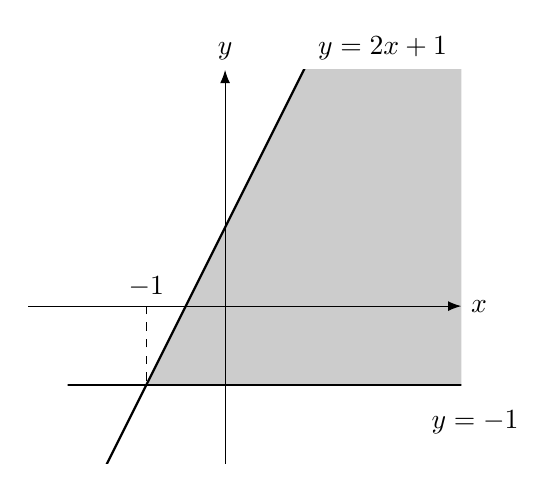
\begin{tikzpicture}

    
    \begin{scope}
        \clip(-2,-2)rectangle(3,3);
        
        \fill[black!20!white]
        plot[domain=3:-1](\x,{0*\x-1})--(-1,-1)--plot[domain=-1:3](\x,{2*\x+1})--cycle;
        \draw[thick]plot(\x,{2*\x+1});
        \draw[thick]plot(\x,{0*\x-1});
        \draw[dashed](0,-1)--(-1,-1)--(-1,0)node[above]{$-1$};

    \end{scope}
    \draw[->,>=Latex](-2.5,0)--(3,0)node[right]{$x$};
    \draw[->,>=Latex](0,-2)--(0,3)node[above]{$y$};
    \node[above]at(2,3){$y=2x+1$};
    \node[below right]at(2.5,-1.2){$y=-1$};
    \end{tikzpicture}   
\end{center}
$\Y Wは上図の網目部で境界をすべて含む.$\\\\
\kakkosanb $C:x^2-4x+y^2-2y+5-a^2\leq0 とする.CがDの部分数集合となるようなaの最大値を求める.$
\begin{align*}
    C:(x-2)^2+(y-1)^2\leq a^2\doti 中心(2,1)半径aの円
    \end{align*}
このことより,次図のとき$a$は最大値を取る.
\begin{center}
    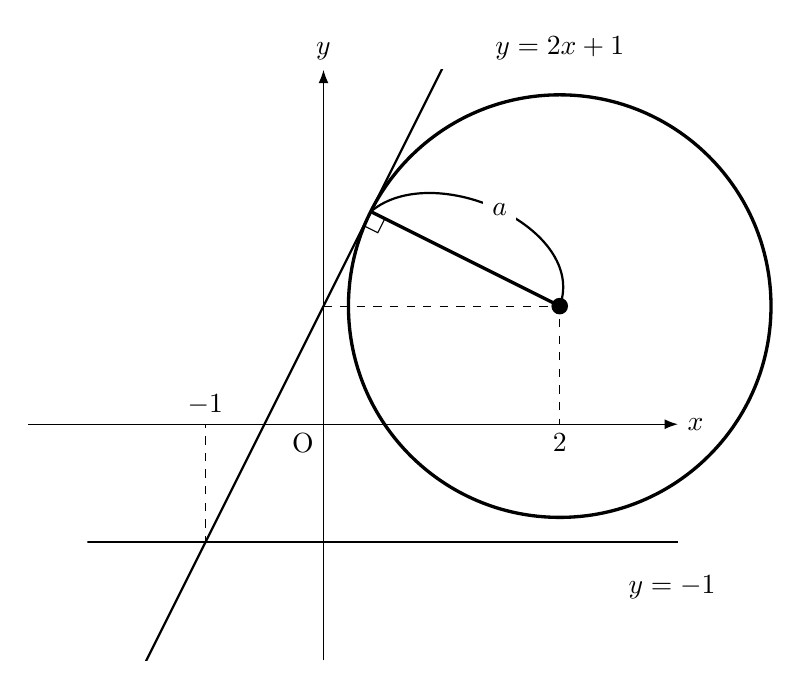
\begin{tikzpicture}[scale=1.5]
        \begin{scope}
        \clip(-2,-2)rectangle(3,3);
        
       
        \draw[thick]plot(\x,{2*\x+1});
        \draw[thick]plot(\x,{0*\x-1});
        \draw[dashed](0,-1)--(-1,-1)--(-1,0)node[above]{$-1$};
        

    \end{scope}
    \draw[->,>=Latex](-2.5,0)--(3,0)node[right]{$x$};
    \draw[->,>=Latex](0,-2)--(0,3)node[above]{$y$};
    \node[above]at(2,3){$y=2x+1$};
    \node[below right]at(2.5,-1.2){$y=-1$};
    \draw[very thick](2,1)circle[radius={4*sqrt(5)/5}];
    \fill(2,1)circle(2pt);
    \draw[dashed](0,1)--(2,1)--(2,0)node[below ]{$2$};
    \coordinate(A)at(0,1);
    \coordinate(B)at(2,5);
    \coordinate(P)at(2,1);
    \coordinate(H)at($(A)!(P)!(B)$);
    \draw[very thick](P)--(H);
    \draw(P)--(H)--(A) pic[draw,angle radius=2mm]{right angle=P--H--A};
    \path [draw,thick] (P) to[out=70,in=40,edge node={node [midway,fill=white]{$a$}}](H);
    \node[below left]at(0,0){O};

    \end{tikzpicture}
\end{center}
$\Y 点と直線の距離公式より,$
\begin{align*}
    a=\dfrac{|4-1+1|}{\sqrt{5}}=\kotaee{\dfrac{4\sqrt{5}}{5}}
\end{align*}\\
\newpage
\noindent\tokenib\\
\kangaekata\\
非常に厄介な確率の問題です.\ans{場合分けが桁違いに多い.}です.\kakkoichib,\kakkonib を完答できていれば御の字です.\\
\kakkosanb では,3回目のBが引くカードがいずれにしても奇数であるということに気づく必要があります.そこからBの3回目のカードの値で場合分けします.\\
\kai\\
まず,A,B$のn回目(1\leq n\leq 3)のときのカードをそれぞれa_n,b_nと表すことにする.$\\
\kakkoichib  $全事象は,6\cdot5\cdot4=120通りである.$\\
ここで,$a=bが成立するのは,$
\begin{align*}
    a_1+a_2=b_1\cdots\cdots\cdots\maruichi
\end{align*}
が成立するときである.\\
\tokeiichi\underline{$b_1=1,2のとき$}\\
 $\maruichi を満たすような(a_1,a_2)は存在しない.$\\
\tokeini\underline{$b_1=3$のとき}\\
 $(a_1,a_2)=(1,2),(2,1)の2通り.$\\
\tokeisan\underline{$b_1=4$のとき}\\
 $(a_1,a_2)=(1,3),(3,1)の2通り.$\\
\tokeishi\underline{$b_1=5$のとき}\\
 $(a_1,a_2)=(1,4),(4,1),(2,3),(3,2)の4通り.$\\
\tokeigo\underline{$b_1=6のとき$}
 $(a_1,a_2)=(1,5),(2,4),(5,1),(4,2)の4通り.$\\
$\Y 以上より,求める確率は,\dfrac{12}{120}=\kotaee{\dfrac{1}{10}}$\\\\
\kakkonib $4枚の札を引くときの全事象は,6\cdot5\cdot4\cdot3=360通りである.$\\
このとき,
\begin{align*}
    a_1+a_2=b_1+b_2(=kとおく.)\cdots\cdots\cdots\maruni \doti kを2通りで表すことができる.
\end{align*}
これより,\\
\tokeiichi\underline{$k\leq4 or k\geq10のとき$}\\
 $\maruni を満たすような(a_1,a_2,b_1,b_2)は存在しない.$\\
\tokeini\underline{$k=5$のとき}\\
 $(a_1,a_2,b_1,b_2)=(1,4,2,3),(2,3,1,4)の\p{2!\times2!}\times2=8通り.$\\
\tokeisan\underline{$k=6$のとき}\\
 $(a_1,a_2,b_1,b_2)=(2,4,1,5),(1,5,2,4)の\p{2!\times2!}\times2=8通り.$\\
\tokeishi\underline{$k=7$のとき}\\
 $3+4 or 1+6 or 2+5 なので,\maruni を満たすような(a_1,a_2,b_1,b_2)の組は,$
\begin{align*}
    \comb{3}{2}\times2\times2\times2&=\B{(a_1,a_2)か(b_1,b_2)の選び方}\times(3+4,1+6,2+5の並び替え)\\
    &=24通り
\end{align*}
\tokeigo\underline{$k=8のとき$}
 $(a_1,a_2,b_1,b_2)=(2,6,3,5),(3,5,2,6)の\p{2!\times2!}\times2=8通り.$\\
\tokeiroku\underline{$k=9のとき$}\\
 $(a_1,a_2,b_1,b_2)=(3,6,4,5),(4,5,3,6)の\p{2!\times2!}\times2=8通り.$\\
$\Y 求める確率は,\dfrac{56}{360}=\kotaee{\dfrac{7}{45}}$\\\\\
\kakkosanb 余事象「6回中少なくとも一回$a=b$」が成立する確率を計算することにより,\kakkosanb の確率を求める.\\
$a=bが実現するのは,3回目以降であり,3回目のと4回目でa=bが成立する確率は\kakkoichib 及び\kakkonib で求めているので,5回目
すなわちa_1+a_2+a_3=b_1+b_2(=\ell とおく.)が成立する確率のみ調べれば良い.$\\
今,$全事象は,6\cdot5\cdot4\cdot3\cdot2=720通りである.$\\
ここで,$a_1+a_2+a_3=(偶数)のとき,a_n,b_n(1\leq n\leq3)の組み合わせは下表の通り.$
\begin{center}
    \begin{tabular}{|c|c|c|c|c|c|c|}
        \hline
        {} & $a_1$ & $a_2$  & $a_3$  & $b_4$ & $b_5$ & $b_6$\\
        \hline
        case1 & き & き & き & ぐ  &ぐ & ぐ\\
        \hline
        case2 &き & き & ぐ & ぐ &ぐ &き\\
        \hline
        case3 &ぐ & ぐ & ぐ& き & き & き\\
        \hline
    \end{tabular}
\end{center}
case1のとき,3つの異なる奇数の和が3つの異なる偶数の和で表すことはできないので,case1は成立しない.\\
次に,$a_1+a_2+a_3=(奇数)のときも同様に考える.$
\begin{center}
    \begin{tabular}{|c|c|c|c|c|c|c|}
        \hline
        {} & $a_1$ & $a_2$  & $a_3$  & $b_4$ & $b_5$ & $b_6$\\
        \hline
        case4 & き & き & き & ぐ  &ぐ & ぐ\\
        \hline
        case5 &き & ぐ & ぐ & き &ぐ &き\\
        \hline
    \end{tabular}
\end{center}
このとき,casem4も同様の理由により不適である.また,いずれのcaseにしても$\ans{b_3は奇数}である.$\\
このことより,$a_1+a_2+a_3+b_1+b_2+b_3=21であり,b_3は奇数であるから,$
\begin{align*}
    a_1+a_2+a_3+b_1+b_2=2m\cdots\cdots\cdots\marusan (m\in\mathbb{N})と表せる.
\end{align*}
\newpage
\noindent このことより,$b_3=1,3,5の場合で場合分けする.$\\
\tokeiichi\underline{$b_3=1$のとき}
 $\ell=10なので,これを満たす(a_1,a_2,a_3)と(b_1,b_2)の組は$
\begin{align*}
    \begin{cases}
        (a_1,a_2,a_3)=(2,3,5)\\
        (b_1,b_2)=(4,6)
    \end{cases}
\end{align*}
なので,$3!\times2!=12通りが満たす.$\\
\tokeini\underline{$b_3=3のとき$}
 $\ell=9なので,これを満たす(a_1,a_2,a_3)と(b_1,b_2)の組は$
\begin{align*}
    \begin{cases}
        (a_1,a_2,a_3)=(1,2,6)\\
        (b_1,b_2)=(4,5)
    \end{cases}
\end{align*}
なので,$12通りがこれを満たす.$\\
\tokeisan\underline{$b_3=5のとき$}\\
 $\ell=8なので,これを満たす(a_1,a_2,a_3)と(b_1,b_2)の組は$
\begin{align*}
    \begin{cases}
        (a_1,a_2,a_3)=(1,3,4)\\
        (b_1,b_2)=(2,6)
    \end{cases}
\end{align*}
なので,$12通りがこれを満たす.$\\
$\Y 以上より,求める確率は,$
\begin{align*}
    1-\p{\dfrac{1}{10}+\dfrac{7}{45}+\dfrac{1}{20}}&=1-\dfrac{1}{5}\p{\dfrac{18+28+9}{36}}\\
    &=\kotaee{\dfrac{25}{36}}
\end{align*}
\newpage
\noindent\tokesanb\\
\kangaekata\\
\kakkonib が漸化式??と思いきや簡単な絶対不等式の問題です.\tokenib に比べたら簡単です!\\
でも絵を描くのは無理だったので参考図(手書き)を添付します.\\
\kai\\
\kakkoichib 図より,
\begin{align*}
    \mathrm{BE}_n&=\dfrac{1}{2}a_n\\
    \mathrm{CE}_n&=3-\dfrac{1}{2}a_n\\
    \mathrm{CF}_n&=\dfrac{1}{2}\p{3-\dfrac{1}{2}a_n}=-\dfrac{1}{4}a_n+\dfrac{3}{2}\\
    \mathrm{AF}_n&=3-\mathrm{CF}_n=\dfrac{a_n}{4}+\dfrac{3}{2}\\
    \mathrm{AD}_{n+1}&=\dfrac{1}{2}\mathrm{AF}_n=\dfrac{a_n}{8}+\dfrac{3}{4}\\
    \mathrm{BD}{_{n+1}}&=3-\mathrm{AD}_{n+1}=-\dfrac{a_n}{8}+\dfrac{9}{4}
\end{align*}
よって,$\mathrm{BD}_{n+1}=a_{n+1}なので,$
\begin{align*}
    a_{n+1}=-\dfrac{1}{8}a_n+\dfrac{9}{4}\doti a_n=2-\p{-\dfrac{1}{8}}^{n-1} (漸化式は暗算でいいよね??)
\end{align*}
$\Y \kotaee{a_2=\dfrac{17}{8},a_3=\dfrac{127}{64}}$\\\\
\kakkonib\begin{align*}
    \left|a_n-2\right|<10^{-9}&\doti \dfrac{1}{8^{n-1}}<10^{-9}\\
    &\doti 2^{-3(n-1)}<10^{-9}\\
    &\doti (n-1)\log_{10}2>3\\
    &\doti n>\dfrac{3}{\log_{10}2}=10.9\cdots\yaku10.9
\end{align*}
$\Y \kotaee{n=11}$
\newpage
\subsection{2024年度実施}
\noindent\tokeichib\\
\kangaekata\\
\kakkonib の連立方程式の計算が煩雑です.同値性を崩さずに正しく場合分けできたでしょうか.確認してください.\\
\kai\\
\kakkoichib $a=1かつb=16のとき$
\begin{align*}
    &\p{\log_2x}^2=\log_24x=2+\log_2x\\
    &\doti \p{\log_2x+2}\p{\log_2x-1}=0\\
    &\doti \log_2x=-2,1\\
    &\doti\kotaee{x=\dfrac{1}{4},2}
\end{align*}\\
\kakkonib $x=2\sqrt{2}を代入すると,$
\begin{align*}
    \p{\log_22\sqrt{2}}^2&=\log_2\p{\sqrt{b}\cdot2\sqrt{2}^a}\\
    &=\dfrac{1}{2}\log_2b+a\log_22^{\frac{3}{2}}
\end{align*}
\begin{align*}
\Y \p{\log_22^{\frac{3}{2}}}^2=\dfrac{1}{2}\log_2b+a\log_22^{\frac{3}{2}}&\doti \p{\dfrac{3}{2}}^2=\dfrac{1}{2}\log_2b+\dfrac{3}{2}a\\
&\doti \dfrac{9}{2}=\log_2b+3a\cdots\cdots\cdots\maruichi 
\end{align*}
$ここで,x=\dfrac{b}{4}を元の式に代入すると,$
\begin{align*}
    \p{\log_2\dfrac{b}{4}}^2=\dfrac{1}{2}\log_2b+a\log_2\dfrac{b}{4}&\doti \p{\log_2b-2}^2=\dfrac{1}{2}\log_2b+a\p{\log_2b-2}\cdots\cdots\cdots\maruni
\end{align*}
さらに$\maruni に\maruichi$ を代入すると,
\begin{align*}
    &\begin{cases}
        \maruichi\\
        \p{\dfrac{9}{2}-3a-2}^2=\dfrac{1}{2}\p{\dfrac{9}{2}-3a}+a\p{\dfrac{9}{2}-3a-2}
    \end{cases}
    \doti
    \begin{cases}
        \maruichi\\
        \p{\dfrac{5}{2}-3a}^2=\dfrac{1}{2}\p{\dfrac{9}{2}-3a}+a\p{\dfrac{5}{2}-3a}
    \end{cases}\\
    &\doti 
    \begin{cases}
        \maruichi\\
        25-60a+36a^2=9-6a+10a=12a^2
    \end{cases}
    \doti
    \begin{cases}
        \maruichi\\
        3a^2-4a+1=0
    \end{cases}\\
    &\doti 
     \begin{cases}
        \maruichi\\
        a=\dfrac{1}{3},1
    \end{cases}
\end{align*}
\newpage
\noindent\tokeiichi\underline{$a=\dfrac{1}{3}$のとき}\\
 $\maruni より,\dfrac{7}{2}=\log_2b\\
 \Y b=2^{\frac{7}{2}}=8\sqrt{2} これより,与式は2\sqrt{2}を重解にもつことになり,\kakkoni の前提に反する.\\
  よって,a\neq\dfrac{1}{3}である.\\
  \tokeini\underline{a=1のとき}\\
   \maruni より,\dfrac{9}{2}=\log_2b+3\doti b=2^{\frac{3}{2}}\\
  このとき,$
  \begin{align*}
    &\p{\log_2x}^2=\log_22^{\frac{3}{4}}\cdot x=\dfrac{3}{4}+\log_2x\\
    &\doti 4\p{\log_2x}^2-4\log_2x-3=0\\
    &\doti \p{2\log_2x-3}\p{2\log_2x+1}=0\\
    &\doti x=2^{\frac{3}{2}},2^{-\frac{1}{2}}\\
    &\doti x=2\sqrt{2},\dfrac{1}{\sqrt{2}}
  \end{align*}  
  これより,$a=1のとき確かに2\sqrt{2}と\dfrac{b}{4}を解に持つ.\\
  \Y \kotaee{a=1,b=2^{\frac{3}{2}}}$ 
  \newpage
  \noindent\tokenib\\
  \kangaekata\\
難易度は高くありませんが計算が煩雑です.落ち着いて計算しましょう.\\
\kai\\
\kakkoichib 参考図を適宜参照せよ.\\
$\begin{cases}
    \theta=30\ddo\\
    \Vec{AP}=\Vec{AC}
\end{cases} のとき,\Vec{EF}\cdot\Vec{EP}=\Vec{EF}\cdot\Vec{EC}である.$
ここで,
\begin{align*}
    \begin{cases}
        \Vec{EF}=\Vec{AF}-\vec{AE}=\dfrac{1}{2}\Vec{AD}-\dfrac{2}{3}\Vec{AB}\\
        \Vec{EC}=\Vec{AC}-\Vec{AE}=\dfrac{1}{3}\Vec{AB}+\Vec{AD}
    \end{cases}
\end{align*}
なので,
\begin{align*}
    k&=\p{\dfrac{1}{2}\Vec{AD}-\dfrac{2}{3}\Vec{AB}}\cdot\p{\dfrac{1}{3}\Vec{AB}+\Vec{AD}}\\
    &=\Vec{AB}\cdot\Vec{AD}\p{\dfrac{1}{6}-\dfrac{2}{3}}+\dfrac{1}{2}\left|\Vec{AD}\right|^2-\dfrac{1}{9}\left|\Vec{AB}\right|^2\\
    &=6\times\dfrac{\sqrt{3}}{2}\times\p{\dfrac{-3}{6}}+\dfrac{1}{2}\times4-\dfrac{2}{9}\times9\\
    &=\kotaee{-\dfrac{3\sqrt{3}}{2}}
\end{align*}\\
\kakkonib Pは直線BC上の点なので,$0\leq t\leq1 をみたすある実数tを用いて,\Vec{AP}=\Vec{AB}+t\Vec{AD}と表せる.$
\begin{align*}
    \Vec{EF}\cdot\Vec{EP}&=\p{\dfrac{1}{2}\Vec{AD}-\dfrac{2}{3}\Vec{AB}}\cdot\p{\Vec{AB}+t\Vec{AD}-\dfrac{2}{3}\Vec{AB}}\\
    &=\p{\dfrac{1}{2}\Vec{AD}-\dfrac{2}{3}\Vec{AB}}\cdot\p{\dfrac{1}{3}\Vec{AB}+t\Vec{AD}}\\
    &=\Vec{AD}\cdot\Vec{AB}\p{\dfrac{1}{6}-\dfrac{2}{3}t}+\dfrac{t}{2}\cdot\left|\Vec{AD}\right|^2-\dfrac{2}{9}\left|\Vec{AB}\right|^2\\
    &=6\cos\theta\times\dfrac{1}{6}(1-4t)+2t-2\\
    &=\cos\theta-2+t\p{2-4\cos\theta}\\
    &=\cos\theta-2+2t\p{1-2\cos\theta}\cdots\cdots\cdots\maruichi (0\leq t\leq1)
\end{align*}
$tが0\leq t\leq 1を満たす任意の値wをとるとき,t=0でも成り立つので$
\begin{align*}
    1-2\cos\theta&\doti \cos\theta=\dfrac{1}{2}\\
    &\doti \kotaee{\theta=\dfrac{\pi}{3}}
\end{align*}
このとき,$\theta=\dfrac{\pi}{3}を\maruichi に代入して,\\
k=\dfrac{1}{2}-2=\kotaee{-\dfrac{3}{2}}$
\newpage
\noindent\kakkosanb $\mathrm{EF}=\mathrm{EP}かつk=-1を満たすとき\mathrm{BP}:\mathrm{PC}の値を求める.$\\
\kangaekata\\
どうしたらいいか判然としないタイプの問題は,とりあえず\ans{与えられた情報を同値変形}しましょう!
\begin{align*}
    \mathrm{EF}=\mathrm{EP}&\doti \left|\Vec{EF}\right|^2=\left|\Vec{FP}\right|^2\\
    &\doti \left|\dfrac{1}{2}\Vec{AD}-\dfrac{2}{3}\Vec{AB}\right|^2=\left|\dfrac{1}{3}\Vec{AB}+t\Vec{AD}\right|^2\\
    &\doti \dfrac{1}{4}\left|\Vec{AD}\right|^2-\dfrac{2}{3}\Vec{AB}\cdot\Vec{AD}+\dfrac{4}{9}\left|\Vec{AB}\right|^2=t^2\left|\Vec{AD}\right|^2+\dfrac{2}{3}t\Vec{AB}\cdot\Vec{AD}+\dfrac{1}{9}\left|\Vec{AB}\right|^2\\
    &\doti 1-4\cos\theta+4=4t^2+4t\cos\theta+1\\
    &\doti 4t^2+4t\cos\theta+4\cos\theta-4=0\\
    &\doti t^2+\cos\theta(t+1)-1=0\cdots\cdots\cdots\maruni 
\end{align*}
一方,$k=-1より$
\begin{align*}
    &-1=\cos\theta-2+2t\p{1-2\cos\theta}\\
    &\doti -1=\cos\theta-2+2t-4t\cos\theta\\
    &\doti \cos\theta(4t-1)=-1+2t\\
    &\doti \cos\theta=\dfrac{2t-1}{4t-1}\cdots\cdots\cdots\marusan
\end{align*}
よって,$\maruni と\marusan より,\marusan を\maruni$ に代入すると
\begin{align*}
    &t^2+(t+1)\cdot\dfrac{2t-1}{4t-1}-1=0\\
    &\doti \dfrac{t^2(4t-1+(t+1)(2t-1)-(4t-1))}{4t-1}=0\\
    &\doti \dfrac{4t^3+t^2-3t}{4t-1}=0\\
    &\doti \begin{cases}
        t(t+1)(4t-3)=0\\
        t\neq\dfrac{1}{4}
           \end{cases}\\
    &\doti t=0,-1,\dfrac{3}{4}\\
    &\doti t=\dfrac{3}{4}
\end{align*}
$\Y t=0のとき,\theta=0となり不適であるので,t=\dfrac{3}{4}である.$\\
$\Y \Vec{AP}=\Vec{AB}+\dfrac{3}{4}\Vec{AD}なので,\kotaee{\mathrm{BP}:\mathrm{PC}=3:1}$
\newpage
\noindent\tokesanb\\
\kangaekata\\
落ち着いて,グラフを描けば大丈夫です.\\
また関数形がややこしいので,$m(x)とM(x)のどっちを採用するのか気をつけましょう.(f(x)とg(x)の上下関係に気を付ける)$\\
\kai\\
\kakkoichib $a=21のとき,m(x)=\begin{cases}
    g(x)=-x^2+8x+9=-(x-9)(x+1)\\
    f(x)=-x^2-4x+21=-(x+7)(x-3)
\end{cases}であり更にf(x)-g(x)=-12x+12=12(1-x)であるから下図の網目部が求める面積である.$
\begin{center}
    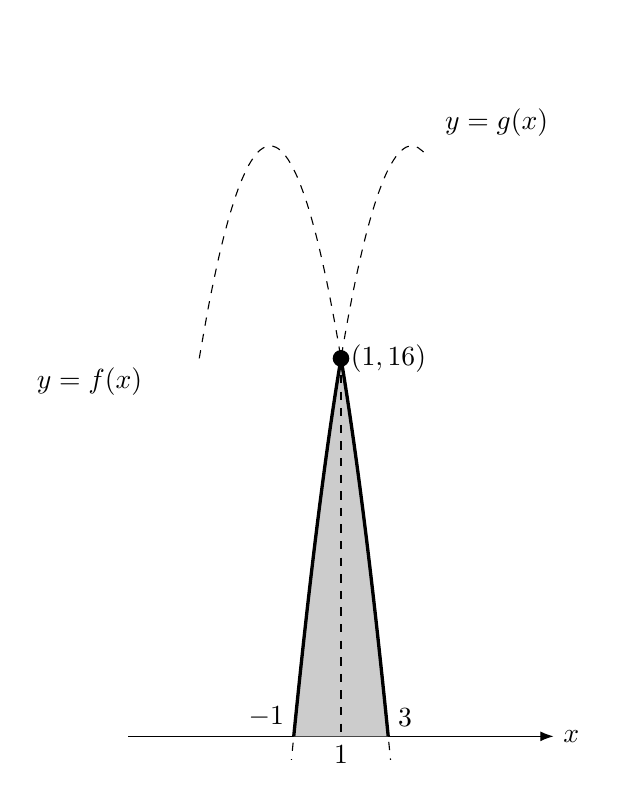
\begin{tikzpicture}[scale=0.3]
        \draw[->,>=Latex](-8,0)--(10,0)node[right]{$x$};
        \coordinate(A)at(1,16);
        \begin{scope}
            \clip(-7.1,-1)rectangle(9.1,30);
            \fill[black!20!white]
            (-1,0)--plot[domain=-1:1](\x,{-pow(\x,2)+8*\x+9})--plot[domain=1:3](\x,{-pow(\x,2)-4*\x+21})--cycle;
        \draw[dashed,smooth]plot(\x,{-pow(\x,2)+8*\x+9});
        \draw[dashed,smooth]plot(\x,{-pow(\x,2)-4*\x+21});
                \end{scope}
                \node[right]at(5,26){$y=g(x)$};
                \node[left]at(-7,15){$y=f(x)$};
                \node[above left]at(-1,0){$-1$};
                \node[above right]at(3,0){$3$};
                \node[right]at(1,16){$(1,16)$};
                \fill(1,16)circle(10pt);
                \draw[very thick,smooth,domain=-1:1]plot(\x,{-pow(\x,2)+8*\x+9});
                \draw[very thick,smooth,domain=1:3]plot(\x,{-pow(\x,2)-4*\x+21});
                \draw[dashed](1,16)--(1,0)node[below]{$1$};
    \end{tikzpicture}
\end{center}
$\Y 求める面積S_1とすると,上図より,$
\begin{align*}
    S_1&=\dint{-1}{1}(-x^2+8x+9)dx+\dint{1}{3}(-x^2-4x+21)dx\\
    &=(頑張って計算\cdots)\\
    &=\kotaee{\dfrac{104}{3}}
\end{align*}\\
\newpage
\noindent\kakkonib $\ell の傾きが2より,y=f(x)とy=g(x)の微分係数をそれぞれ計算することにより,$
\begin{align*}
    \begin{cases}
        g^\prime(x)=-2x+8\\
        f^\prime(x)=-2x-4
    \end{cases}&\doti\begin{cases}
        2=-2x+8\\
        2=-2x-4
    \end{cases}\\
    &\doti\begin{cases}
        x=3 (\ell とy=g(x)の接点のx座標)\\
        x=-3 (\ell とy=f(x)の接点のx座標)
    \end{cases}
\end{align*}
よって,$このとき\ell の方程式は,$
\begin{align*}
    \ell:y=2(x-3)+24=2x+18
\end{align*}
これより,$x=-3のとき,f(-3)=12を満たすので,$
\begin{align*}
    -9+12+a=12\doti\kotaee{a=9}
\end{align*}
$\Y M(x)=\begin{cases}
    -x^2-4x+9 (f(x)\geq g(x))\\
    -x^2+8x+9 (f(x)<g(x))
\end{cases}\\
f(x)とg(x)の交点のx座標は,f(x)=g(x)\doti x=0 である.$\\
従って,$求める面積S_2とすると,それは次図の網目部である.$
\begin{center}
    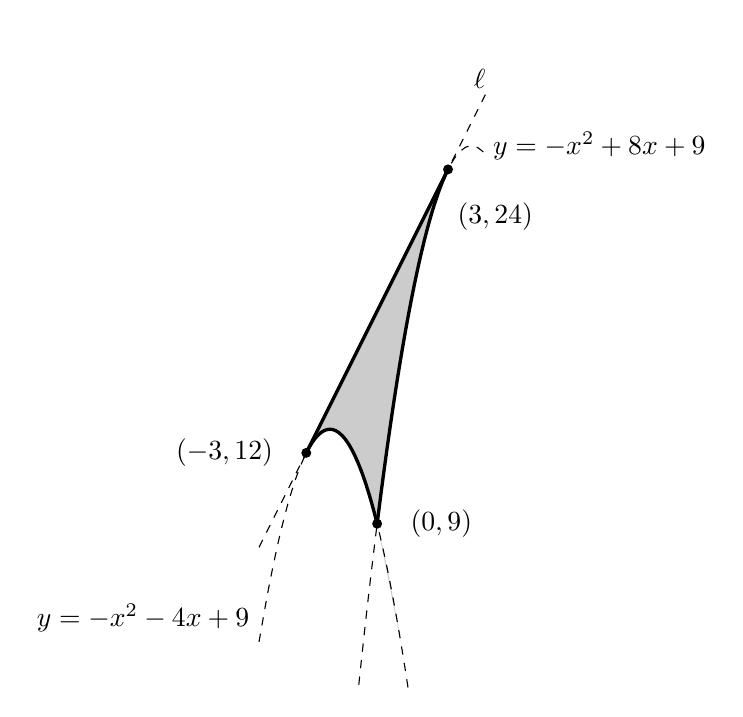
\begin{tikzpicture}[scale=0.3]
        \coordinate(A)at(0,9);
        \begin{scope}
            \clip(-6,2)rectangle(8,30);
            \fill[black!20!white]
            (A)--plot[domain=0:3](\x,{-pow(\x,2)+8*\x+9})--plot[domain=3:-3](\x,{2*\x+18})--plot[domain=-3:1](\x,{-pow(\x,2)-4*\x+9})--cycle;
        \draw[dashed,smooth]plot(\x,{-pow(\x,2)+8*\x+9});
        \draw[dashed,smooth]plot(\x,{-pow(\x,2)-4*\x+9});
        \draw[dashed,smooth]plot(\x,{2*\x+18});
                \end{scope}
                \draw[very thick,smooth,domain=0:3]plot(\x,{-pow(\x,2)+8*\x+9});
                \draw[very thick,smooth,domain=-3:0]plot(\x,{-pow(\x,2)-4*\x+9});
                \draw[very thick,smooth,domain=3:-3]plot(\x,{2*\x+18});
                \fill(3,24)circle(6pt);
                \fill(-3,12)circle(6pt);
                \node[above left]at(-4,11){$(-3,12)$};
                \node[above left]at(-5,4){$y=-x^2-4x+9$};
                \node[above right]at(4.5,24){$y=-x^2+8x+9$};
                \node[below]at(5,23){$(3,24)$};
                \node[above left]at(5,27){$\ell$};
                \fill(0,9)circle(6pt);
                \node[right]at(1,9){$(0,9)$};

    \end{tikzpicture}
\end{center}
上図より,$S_2は,$
\begin{align*}
    S_2&=\dint{-3}{0}\B{2x+18-\p{-x^2-4x+9}}dx+\dint{0}{3}\B{2x+18-\p{-x^2+8x+9}}dx\\
    &=(頑張って計算)\\
    &=\kotaee{18}
\end{align*}
\newpage
\subsection{2025年度実施}
\noindent\tokeichib\\
\kangaekata\\
1次元数直線上の解の個数の問題です.\ans{共通部分なのか合併集合なのか}を意識して解けば間違えるところはありません.(合併集合=合わせた部分)\\
\kai
\begin{align*}
\begin{cases}
    2x^2-4bx+15b=0\cdots\cdots\cdots\maruichi\\
    x^2+8x+b+15=0\cdots\cdots\cdots\maruni
\end{cases}
\end{align*}
$\maruichi,\maruni の判別式をそれぞれD_1,D_2とおく.$\\
\kakkoichib $a=5のとき$
\begin{align*}
    \begin{cases}
        \maruichi\\
        \maruni
    \end{cases}\doti\begin{cases}
        2x^2-4bx+15b=0\\
        x^2+8x+b+15=0
    \end{cases}
\end{align*}
なので,
\begin{align*}
    \begin{cases}
        D_1=4b^2-30b=0\\
        D_2=16-b-15\geq0
    \end{cases}&\doti \begin{cases}
        b(2b-15)=0\\
        b\leq1
    \end{cases}\\
    &\doti \kotaee{b=0}
\end{align*}\\
\kakkonib $D_1,D_2を計算すると,$
\begin{align*}
    \begin{cases}
    D_1=4b^2-6ab=0\\
    D_2=a^2-4a-6\geq0
    \end{cases}&\doti \begin{cases}
        2b(2b-3a)=0\\
        a^2-4a-6\leq0
    \end{cases}\\
    &\doti \begin{cases}
        b=0 or b=\dfrac{3}{2}a\\
        a^2-4a-6\leq0
    \end{cases}
\end{align*}
これより,\\
$\bullet$ \underline{$b=0のとき$}\\
 $a^2-4a-6\leq0\doti 2-\sqrt{10}\leq a\leq2+\sqrt{10}\cdots\cdots\cdots\marusan $\\
$\bullet$ \underline{$b=\dfrac{3}{2}aのとき$}
 \begin{align*}
    a^2-4a-6+\dfrac{3}{2}a\leq0&\doti 2a^2-5a-12\leq0\\
    &\doti (2a+3)(a-4)\leq0\\
    &\doti -\dfrac{3}{2}a\leq a\leq4\cdots\cdots\cdots\marushi 
\end{align*}
また,$a=\dfrac{2}{3}aよりbの取りうる値の範囲は,-\dfrac{a}{4}\leq b\leq6\cdots\cdots\cdots\marugo$\\
$\Y aの取りうる値の範囲は,\marusan と\marushi を合わせた範囲なので,\kotaee{-\dfrac{3}{2}\leq a\leq 2\sqrt{10}}\\
\Y bの取りうる値の範囲は,\marugo とb=0を合わせた範囲なので,\kotaee{-\dfrac{9}{4}\leq b\leq6}$\\\\
\kakkosanb $-\dfrac{3}{2}\leq a\leq 2\sqrt{10}または-\dfrac{9}{4}\leq b\leq6を満たすa,bの個数を数えれば良い.\\
まず,-\dfrac{3}{2}\leq a\leq 2\sqrt{10}を満たすaは,a=-1,0,1,2,3,4,5の計7個.\\
次に,-\dfrac{9}{4}\leq b\leq6を満たすbは,b=-2,-1,0,1,2,3,4,5,6の計9個.\\
\Y 求める(a,b)の組の個数は\kotaee{9個}.$
\newpage
\noindent\tokenib\\
\kangaekata\\
完答意外ない.\\
\kai\\
\kakkoichib 玉を2回取り出してOにいる確率は,$\p{\dfrac{1}{4}\times\dfrac{1}{4}\times2}\times2=\kotaee{\dfrac{1}{4}}\\\\
\kakkonib  玉を3回取り出して\mathrm{P}が(1,0)にいるとき,$
\begin{align*}
    \to\uparrow\downarrow,\to\to\leftarrow
\end{align*}
の2通りなので,求める確率は,  $3!\cdot\p{\dfrac{1}{4}}^3+\dfrac{3!}{2!}\p{\dfrac{1}{4}}^3=\kotaee{\dfrac{9}{64}}$\\\\
\kakkosanb 玉を4回取り出してPが$(1,1)にいるとき,$
\begin{align*}
    \yaa\to\leftarrow,\yaa\uparrow\downarrow 
\end{align*}
であり,$\yaa =\to \uparrow であることに注意して,$求める確率は,$\dfrac{4!}{2!}\times2\times\p{\dfrac{1}{4}}^4=\kotaee{\dfrac{3}{32}}$
\newpage
\noindent\tokesanb\\
\kangaekata\\
対称性:$y=f(-x)=-f(x)であり,-y=f(x)なので,y=f(x)のグラフは原点について対称です.これで積分計算を楽に済ませることができます.$\\
\kai\\
$f(x)=3x^3-(a+1)^2x=x\B{\sqrt{3}x+\p{a+1}}\B{\sqrt{3}x-\p{a+1}}と因数分解でき,更に(x,y)=(-x,-y)とすると,y=f(x)なので,y=f(x)のグラフは
原点について対称である.$\\
また,$\alpha=-\dfrac{a+1}{\sqrt{3}},\beta=\dfrac{a+1}{\sqrt{3}}(\alpha<\beta)とおく.$\\
\kakkoichib 対称性より,
\begin{align*}
    \dfrac{27}{2}=2\times\dint{0}{\beta}(-f(x))dx\cdots\cdots\cdots\maruichi 
\end{align*}
である.\\
ここで,
\begin{align*}
    -\dint{0}{\beta}f(x)dx&=\dint{\beta}{0}\B{3x^3-\p{a+1}^2x}dx\\
    &=\dfrac{3}{4}\tint{x^4}{\beta}{0}-\dfrac{(a+1)^2}{2}\tint{x^2}{\beta}{0}\\
    &=-\dfrac{3}{4}\cdot\dfrac{(a+1)^4}{9}+\dfrac{(a+1)^4}{6}\\
    &=(a+1)^4\cdot\dfrac{1}{12}
\end{align*}
よって,
\begin{align*}
     \dfrac{1}{6}(a+1)^4=\dfrac{27}{2}&\doti (a+1)^4=3^4\\
     &\doti a+1=3\\
     &\doti \kotaee{a=2}
\end{align*}\\
\kakkonib $f^\prime(x)=9x^2-(a+1)^2=9\p{x+\dfrac{a+1}{3}}\p{x-\dfrac{a+1}{3}} より,次の増減表を得る.$
\begin{center}
    \begin{tabular}{|c||c|c|c|c|c|}
        \hline
        $x$ & $\cdots$ & $-\dfrac{a+1}{3}$ & $\cdots$ & $\dfrac{a+1}{3}$ & $\cdots$\\
        \hline
        $f^\prime(x)$ & $+$ & $0$ & $-$ & $0$ & $+$\\
        \hline
        $f(x)$ & $\yaa$ & $極大$ & $\yab$ & $極小$ & $\yaa$\\
        \hline
    \end{tabular}
\end{center}
$よって,p=-\dfrac{a+1}{3}なので,極大値はf(p)=3p^3-(a+1)^2p であるから(p,f(p))の軌跡をWとすると,X=p,Y=f(p)とおけて,$
\begin{align*}
    (X,Y)\in W&\doti \exists p,\begin{cases}
        p=X\\
        Y=3p^3-(a+1)^2p
    \end{cases}\\
    &\doti\exists a,\begin{cases}
        Y=3X^3-(a+1)^2X\\
        a+1=-3X
    \end{cases}\\
    &\doti\begin{cases}
        Y=3X^3-9X^3=-6X^3\cdots\cdots\cdots\maruni\\
        a>0
    \end{cases}\\
    &\doti\begin{cases}
        -3X-1>0\\
        \maruni
    \end{cases}\\
    &\doti\begin{cases}
        X<-\dfrac{1}{3}\\
        \maruni
    \end{cases}
\end{align*}
$\Y Wは,\begin{cases}
    y=-6x^3\\
    x<-\dfrac{1}{3}
\end{cases}で,次図の太実線部である.ただし,白丸は含まない.$
\begin{center}
    \begin{tikzpicture}
        \draw[->,>=Latex](-3,0)--(3,0)node[right]{$x$};
        \draw[->,>=Latex](0,-3)--(0,3)node[above]{$y$};
        \draw[smooth,dashed,domain=-1:1.4]plot(\x,{-pow(\x,3)})node[right]{$y=-6x^3$};
        \begin{scope}
            \clip(-1.5,0.5)rectangle(0,5);
            \draw[very thick,smooth]plot(\x,{-pow(\x,3)});
            
        \end{scope}
        
        \draw[dashed]({-1*1/sqrt(2)-0.1},0)--({-1*1/sqrt(2)-0.1},{1/2})--(0,{1/2})node[right]{$\frac{2}{9}$};
        \filldraw[very thick,fill=white,draw=black]({-1*1/sqrt(2)-0.1},{1/2})circle(2pt);
        \node[below]at({-1*1/sqrt(2)-0.1},0){$-\frac{1}{3}$};
        \node[below right]at(0,0){O};
    \end{tikzpicture}
\end{center}
\end{document}
